\documentclass[a4paper,12pt]{article} 
\usepackage[includehead]{geometry}   
\usepackage[utf8]{inputenc}  

\usepackage[german]{babel}
\usepackage{csquotes}
\usepackage{listings}

\usepackage{amsmath}

%linespacing
\usepackage[onehalfspacing]{setspace}

%kopfzeile
\usepackage{fancyhdr}
\pagestyle{fancy}
\fancyhf{}
\fancyhead[R]{\thepage}                         % Kopfzeile rechts bzw. außen
\renewcommand{\headrulewidth}{0.5pt}            % Kopfzeile rechts bzw. außen

%footnote
\interfootnotelinepenalty=10000

%images
\usepackage{float}
\usepackage{subfig}
\usepackage{graphicx}
\graphicspath{ {images/} }

%acronym
\usepackage[nohyperlinks, printonlyused]{acronym}

%todo
\usepackage[textsize=tiny]{todonotes}
%diagonalbox
\usepackage{diagbox}

\usepackage{array}
\usepackage{longtable}
\usepackage{rotating}
\usepackage{graphicx}
\usepackage{makecell, caption, booktabs}
\usepackage[inkscapeformat=png]{svg}
\usepackage{listings}
\usepackage{xcolor}
\usepackage{enumitem}
\usepackage{spverbatim}
\usepackage{lscape}
% nicer c++
\newcommand{\cpp}{C\texttt{++} }

%references
\usepackage[backend=bibtex,style=numeric,sorting=none]{biblatex}
\addbibresource{literatur/literatur.bib}

\DeclareCiteCommand{\citep}
{(vgl. [\usebibmacro{cite}]}{}{}{, \usebibmacro{postnote})}
\DeclareCiteCommand{\citew}
{(vgl. [\usebibmacro{cite}]}{}{}{)}

%plotting
\usepackage{pgfplots}
\pgfplotsset{compat=1.17}

%table
\usepackage{tabularx}

%clickable references
\usepackage{hyperref}
\hypersetup{
    colorlinks,
    citecolor=black,
    filecolor=black,
    linkcolor=black,
    urlcolor=black
}
% makecell
\usepackage{makecell}
\usepackage{multirow}

% section
\newcommand{\nonumsection}[1]{
  \phantomsection
  \addcontentsline{toc}{section}{#1}
  \section*{#1}
}
\newcommand{\nonumcontent}[1]{
  \phantomsection
  \addcontentsline{toc}{section}{#1}
}
\newcommand{\nonumtoc}[1]{
	\phantomsection
	\section*{#1}
}

% math commands
\newcommand{\floor}[1]{\left\lfloor #1 \right\rfloor}

% page numbering
\newcounter{savepagenumber}
\newcommand\frontmatter{
    \cleardoublepage
    \pagenumbering{roman}
    \setcounter{page}{1}
}

\newcommand\mainmatter{
    \cleardoublepage
    \setcounter{savepagenumber}{\value{page}}
    \pagenumbering{arabic}
}
\newcommand\backmatter{
    \clearpage
    \pagenumbering{roman}
    \setcounter{page}{\value{savepagenumber}}
}

%%%%%%%%%%%%%%%%%%%%%%%%%%%%%%%%%%%%%%%%%%%%%%%%%%%%%%%%%%%%%%%%%%%%%%%%%%%%%%%%%%%
\def\myTopic{Erstellung der Hard- und Software zur Steuerung der Segel im Sailwind 4 Projekt}
\def\myAutor{Nico Finkbeiner}
\def\myEndDate{31.12.2023}
\def\myEndPlace{Konstanz}
\def\myMatrikelnummer{298837}
\def\myKurs{TIT20}
\def\myAutorTwo{Benedikt Horn}
\def\myMatrikelnummerTwo{300889}

\def\mySupervisor{Prof. Dr. Dieter Schwechten}
\def\mySupervisorTwo{Prof. Dr. Boris Böck}
%%%%%%%%%%%%%%%%%%%%%%%%%%%%%%%%%%%%%%%%%%%%%%%%%%%%%%%%%%%%%%%%%%%%%%%%%%%%%%%%%%%

%dokument
\begin{document}
	\pagestyle{fancy}
	\addtocontents{toc}{\vspace{0.125 cm}}
	\fancyhead[L]{\nouppercase{\leftmark}}

    \begin{titlepage}
\vspace*{-3cm}
    \begin{figure}[ht]
        \hspace{7cm}\subfloat{{
\includegraphics[width=11cm]{images/Logo/HTWG_Logo.png} }}
    \end{figure}
        
	\begin{center}
		\vspace*{1cm}
		\LARGE\bf\myTopic\\
		\vspace*{1cm}
		\normalsize\rm
		\vspace*{1cm}
		\textbf{Projektarbeit}\\
		\vspace*{0.5cm}
		An der Fakultät Elektro- und Informationstechnik \\
		\vspace*{0.5cm}
		vorgelegt von  \\
	    \vspace*{0.25cm}
		\textbf{Benedikt Horn und Nico Finkbeiner}  \\
		\vspace*{0.25cm}
		Matrikelnummer: 300889 und \myMatrikelnummer \\
		\vspace*{1cm}
		Hochschule Konstanz für Technik, Wirtschaft und Gestaltung \\
		\vspace*{1cm}
		Hochschulbetreuer: \\
		\textbf{\mySupervisorTwo}\\
		\textbf{\mySupervisor}\\
		\vspace*{1cm}
		\textbf{Konstanz den \today}
	\end{center}
\end{titlepage}
\newpage
\setcounter{page}{2}


    \onehalfspacing

    \frontmatter %-------------------------------------------------

    \include{pages/erklärung}
    \nonumsection{Kurzfassung}

\thispagestyle{empty}
\newpage

\section*{Abstract}


    \newpage
\tableofcontents
    \include{pages/abkürzungsverszeichnis}
    \nonumcontent{Abbildungsverzeichnis}
\listoffigures

    \nonumcontent{Quellcodeverzeichnis}
\renewcommand{\lstlistlistingname}{Quellcodeverzeichnis}

\definecolor{codegray}{rgb}{0.5,0.5,0.5}
\definecolor{backcolour}{rgb}{0.95,0.95,0.92}

\lstdefinestyle{mystyle}{
  frame = single,
  backgroundcolor=\color{backcolour}, commentstyle=\color{codegreen},
  basicstyle=\ttfamily\footnotesize,
  captionpos=b,
}
\lstset{style=mystyle}
\lstlistoflistings

\definecolor{eclipseStrings}{RGB}{42,0.0,255}
\definecolor{eclipseKeywords}{RGB}{127,0,85}
\colorlet{numb}{magenta!60!black}

\lstdefinelanguage{json}{
	basicstyle=\normalfont\ttfamily,
	commentstyle=\color{eclipseStrings}, % style of comment
	stringstyle=\color{eclipseKeywords}, % style of strings
	numbers=left,
	numberstyle=\scriptsize,
	stepnumber=1,
	numbersep=8pt,
	showstringspaces=false,
	breaklines=true,
	frame=lines,
	backgroundcolor=\color{backcolour}, %only if you like
	string=[s]{"}{"},
	comment=[l]{:\ "},
	morecomment=[l]{:"},
	literate=
	*{0}{{{\color{numb}0}}}{1}
	{1}{{{\color{numb}1}}}{1}
	{2}{{{\color{numb}2}}}{1}
	{3}{{{\color{numb}3}}}{1}
	{4}{{{\color{numb}4}}}{1}
	{5}{{{\color{numb}5}}}{1}
	{6}{{{\color{numb}6}}}{1}
	{7}{{{\color{numb}7}}}{1}
	{8}{{{\color{numb}8}}}{1}
	{9}{{{\color{numb}9}}}{1}
}
    
    \mainmatter %------------------------------------------------

        \nonumsection{Vorbemerkung}
In der folgenden Arbeit wird aus Gründen der besseren Lesbarkeit ausschließlich die männliche Form verwendet. Sie bezieht sich auf alle Geschlechter gleichermaßen.
\newpage
        \section{Einleitung}
\subsection{Ausgangssituation}

\subsection{Ziel}
\newpage




        \section{Grundlagen zur Segeleinstellung}\label{sec:principles}
In diesem Kapitel wird grob auf die Bedeutung und Funktionsweise der Segelsteuerung eingegangen. Nachfolgende Informationen basieren auf dem Wissensstand der Vorgruppe, in deren Arbeit auf genauere Details zu dieser Thematik verwiesen wird. Eine Skizze, die daraus entnommen wurde, veranschaulicht den Sachverhalt des Segelanstellwinkels:
\begin{figure}[H]
	\centering
	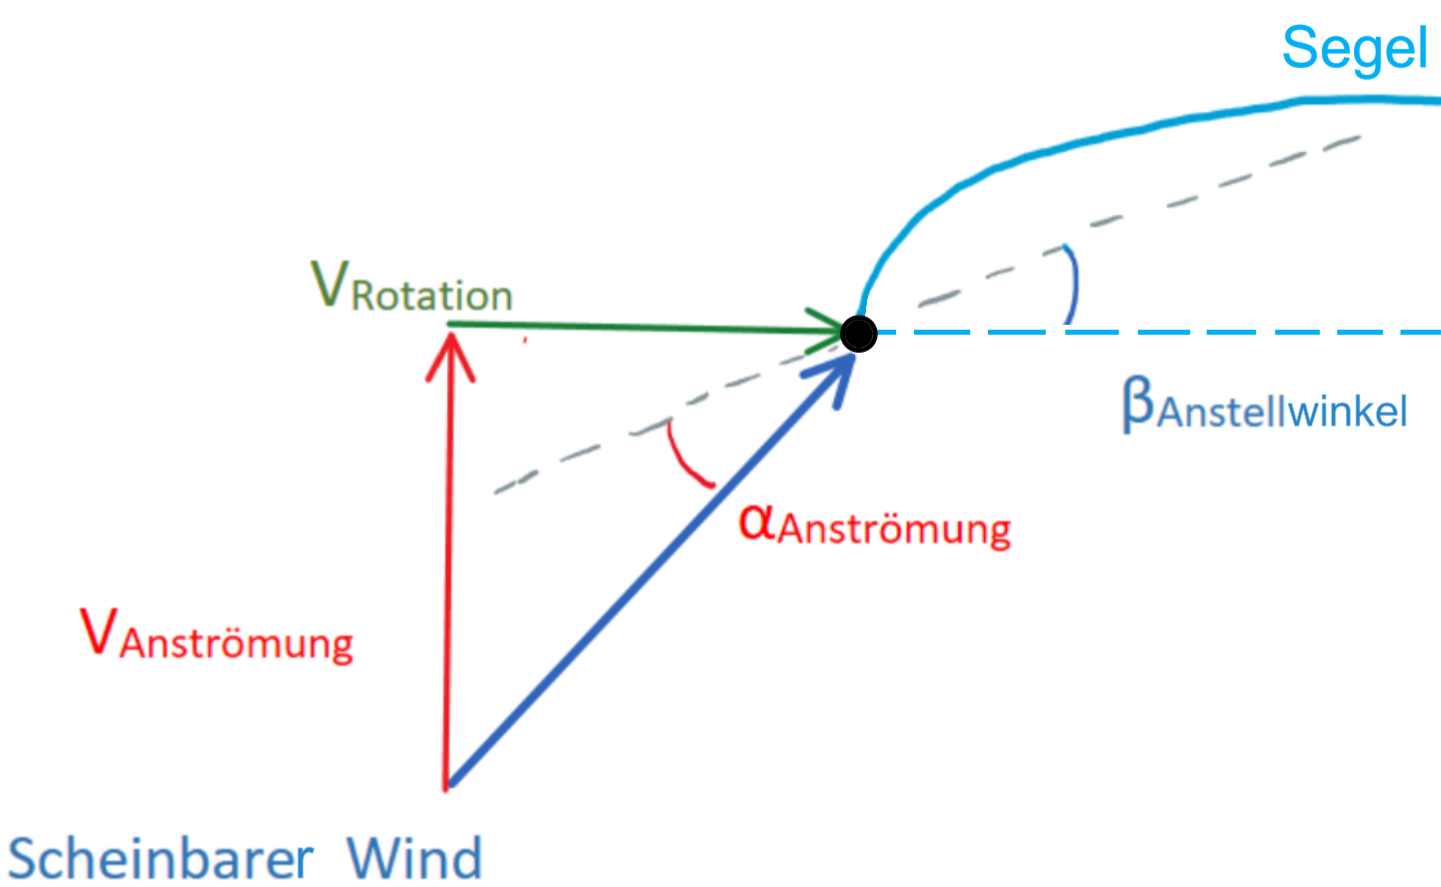
\includegraphics[width=0.6\textwidth]{images/Sailwind/sailPitchAngle.png}
	\caption{Segeltheorie: Scheinbarer Wind und Anstellwinkel}
	\label{fig:sailPitch}
\end{figure}
\noindent
Bei einem Segelboot beeinflusst der Fahrtwind den wahren Wind (hier \textit{Anströmung}) zu einem scheinbaren Wind, der effektiv in das Segel bläst. Ähnlich verhält es sich bei einem in diesem Fall segelartigen Rotorblatt, dass den Wind durch die erzeugte Rotation ablenkt. Verändert sich die Anströmungsgeschwindigkeit, muss der Anstellwinkel des Segels entsprechend angepasst werden, sodass der resultierende scheinbare Wind möglichst effizient vom Segel aufgenommen und in Rotation umgewandelt wird. So existiert zu jeder Windgeschwindigkeit ein optimaler Anstellwinkel. Diese Anpassung wird auch als Trimmen des Segels bezeichnet.\\

\noindent
Wie bereits in der Einleitung erwähnt soll bei einer Windgeschwindigkeit von 14 m/s eine Leistung von 5 kW erzeugt werden. Damit diese auch bei stärkerem Wind konstant abrufbar ist, soll die Segelfläche durch Einrollen verkleinert werden. \autoref{fig:powerCurve} zeigt die erwartete Leistungskurve in Abhängigkeit der Windstärke bei gezielter Trimmung und Rollung der Segel:
\begin{figure}[H]
	\centering
	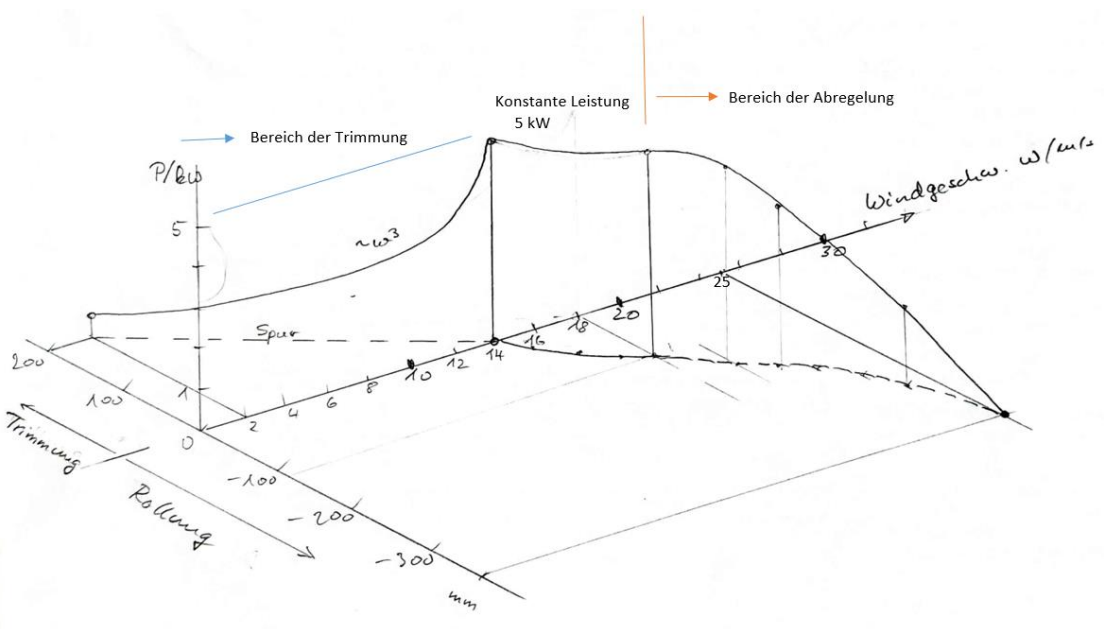
\includegraphics[width=1.0\textwidth]{images/Sailwind/powerCurve.png}
	\caption{SAILWIND Leistungskurve nach Prof. Schwechten}
	\label{fig:powerCurve}
\end{figure}
\noindent
Die Seilführung der Segel (siehe \autoref{fig:sailWindMill}) ermöglicht dabei einen fließenden Übergang zwischen Rollung und Trimmung durch eine gemeinsame Zugbewegung aller Seile parallel zur Rotorwelle, die mithilfe der Linearführung ausgeführt werden soll. Bei einer Einschaltgeschwindigkeit von 1 bis 2 m/s sollen die Segel vollständig getrimmt und ausgerollt sein. Bis zur Nenngeschwindigkeit von 14 m/s befindet sich das System im Teillastbereich, in dem der Anstellwinkel schrittweise reduziert werden soll, um stets die optimale Leistung herauszuholen. Mit weiterem Anstieg der Windgeschwindigkeit beginnt der Volllastbereich, in dem die Segel immer weiter eingerollt werden, um die Spitzenleistung von 5 kW zu erhalten. Ab einem kritischen Wert von ca. 18 m/s soll ein Abregelungsprozess durchgeführt werden.   
        \section{Hardware}
\begin{figure}[H]
	\centering
	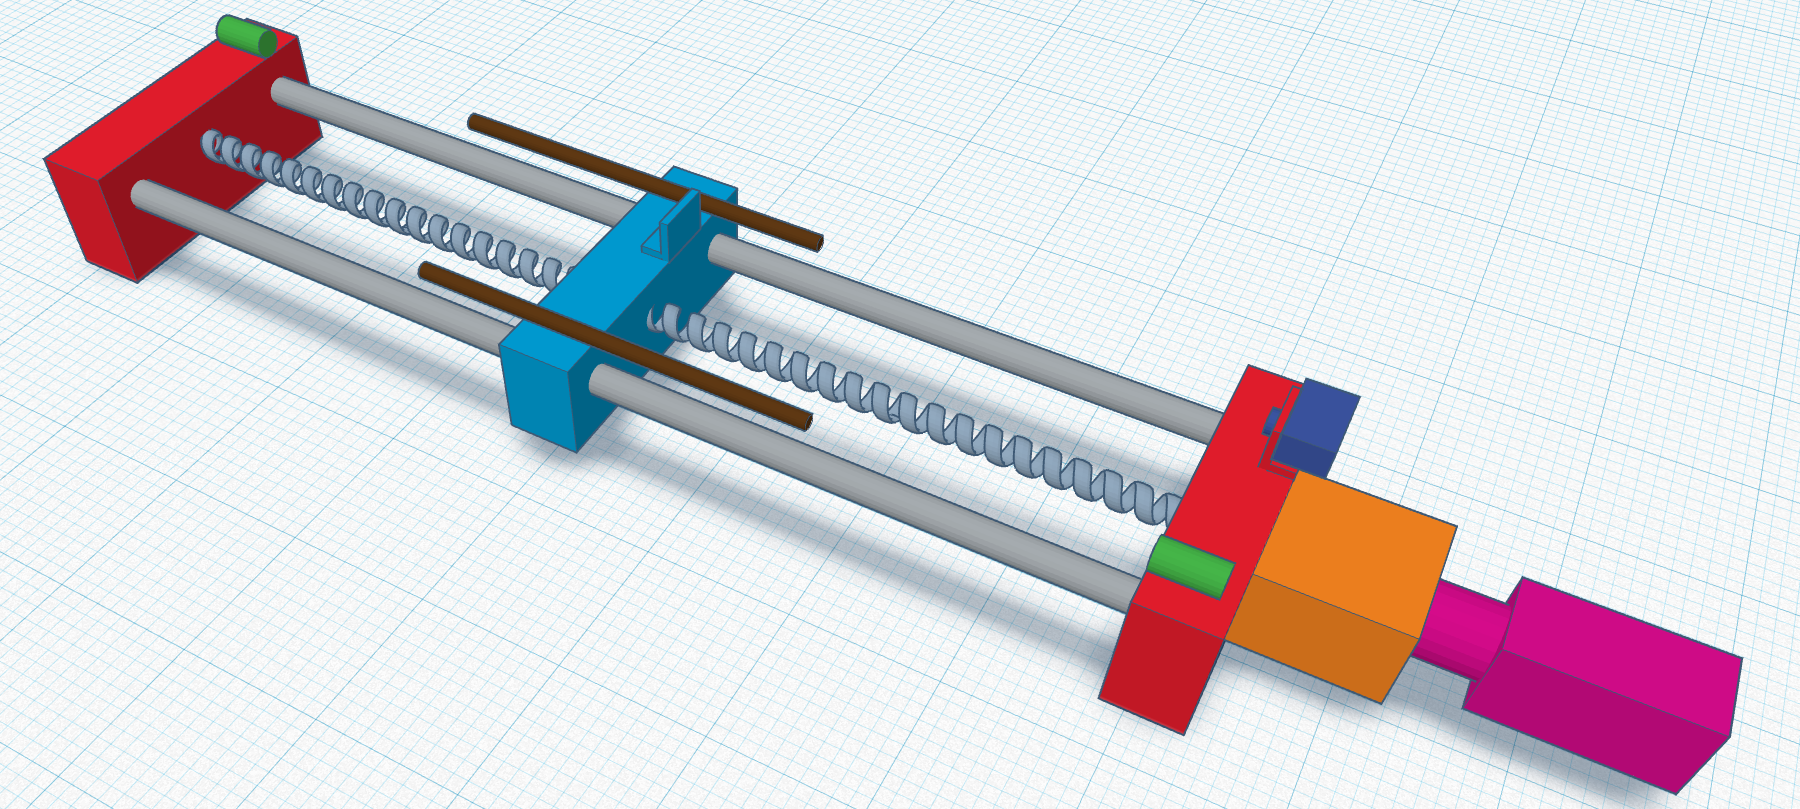
\includegraphics[width=1.0\textwidth]{images/Hardware/Linerarfuerhrung_3D_Modell.png}
	\caption{Simplifiziertes 3D Modell der Lineraführung}
	\label{fig:Systemaufbau}
\end{figure}
Da sich das Sailwind 4.0 Projekt noch in der Entwicklung befindet, existiert noch kein komplett Zusammengebauter Prototyp in dem alle Teile des Projektes zusammenfinden. Die für diese Arbeit relevante Linearführung ist bereits als eigenstehendes Objekt zusammengebaut und wie in \autoref{fig:Systemaufbau} zusehen, aufgebaut. Dabei wird die rotierende Bewegung eines BLDC Motors (Pink) mit der Hilfe eines Getriebes (Orange) und einer Gewindestange in eine Translatorische Bewegung umgewandelt, mit der der Schlitten (Hellblau) zwischen den beiden Stationären Punkten (Rot) hin und her bewegt werden kann. Die beiden Endschalter (Grün) dienen als Kollisionserkennung und können auch genutzt werden um den Bewegungsraum einzuschränken. Dabei können zwei Metallstangen (Braun) verschoben werden und geben damit vor wie viel Platz zwischen dem Schlitten und dem Stationären Elementen bleibt. Zusätzlich kann über einen Abstandssensor (dunkel Blau) die Position des Schlittens in Relation zum Abstandssensor bestimmt werden.\\

\noindent Die Linearführung soll später dazu genutzt werden um die Segel des Windkraftwerkes zu Trimmen und zu Rollen (siehe \autoref{???}). Zusätzlich zu dem präsentierten Aufbau soll sich auf dem Schlitten später ein Druckkraftsensor befinden der die Kraft auf die Rotorwelle messen soll. Dieser wurde allerdings zum Zeitpunkt der Arbeit noch nicht geliefert oder auf dem Prototypen angebracht. Getrennt vom Aufbau soll ebenfalls ein Anemometer an der Kuppel angebracht werden, das die Windrichtung und Geschwindigkeit misst.

%Hier erwähnen was Platine alles für Aufgaben hat
%Um die Segel des Windkraftwerkes jederzeit für maximale Effizienz eingestellt zu haben, müssen diese dynamisch Eingestellt werden können. Hierfür überwacht ein Controllino, die über Sensoren seine Umgebung und berechnet daraus die optimale Segel Einstellung. (KP sollte besser schon früher erwähnt werden/bzw wurde eventuell schon erwähnt)
\subsection{Ziele}
Die Hardware der Steuerung zu der eben vorgestellten Linearführung soll dabei folgende Aufgaben übernehemen:
\begin{itemize}
	\item Ansteuerung aller Sensoren und Aktoren
	\item Stromversorgung aller Komponenten
	\item Lokale Bedienung der Steuerung
	\item Ethernetkommunikation mit dem Controllino
\end{itemize}

\noindent Neben diesen Aufgaben soll die ganze Steuerung in einem zumindest Staub- und Spritzwassergeschützen Gehäuse untergebracht werden. Eine Vorgänger Gruppe hatte sich dieser Aufgabe bereits gewidmet, allerdings war der resultierende Prototyp leider nicht weiter verwendbar und hatte auch einen zu großen Formfaktor. Diese Probleme sollen in dieser Iteration ebenfalls behoben werden.

%Bei dem Entwurf der Hardware sind mehrere Dinge zu beachten. Da das Sailwind 4.0 Projekt noch in den Startschuhen steht, sind einige dieser Faktoren auch noch nicht klar Bestimmbar zum Zeitpunkt dieser Arbeit. Aus diesem Grund wurden an manchen Stellen die Design Kriterien freier oder unnötig Komplex ausgelegt.\\
%
%Um die Steuerung der Segel zu ermöglichen wird ein System benötigt das alle nötigen Akteure und Sensoren, Ansteuret und Überwacht. Hierfür soll eine Steuerelektronik Hardware entworfen werden. Da sich diese im Außeneinsatz befindet sollte diese in einem Wasserdichten Gehäuse eingeschlossen sein. Eine vorrausgehende Gruppe hatte bereits die Steuerelektronik entworfen, diese war allerdings zu groß dimensioniert und hatte einige Fehler, weswegen ebenfalls ein kleinere Formfaktor und die Behebung der Probleme als Ziel gesetzt wurden. Die Steuerelektronik soll Manuell Bedienbar sein, wewegen am Gehäuse ebenfalls eine Bedienmöglichkeit existieren sollte.

\label{Analyze_der_Aktoren_und_Sensoren}
\subsection{Analyse der bestehenden Hardware Elemente}
Um eine geeignete Steuerplatine zu entwerfen, bedarf es einer Analyse der anzusteurenden Hardware Komponenten. Diese wurden bereits von vorrausgehend Gruppen festgelegt. Diese können in die Kategorien Sensoren und Aktoren gruppiert werden. Dabei wurden die benötigte Spannung, die Stromstärke und die Schnittstellen betrachtet. Durch die Spannung und die Stromaufnahme kann später die benötigte Spurenbreite auf der Platine bestimmt werden. Die Schnittstellen geben an wie mit dem jeweiligen Gerät kommuniziert werden kann und welche davon benötigt werden.\\

\subsubsection{Sensoren}
Zu den Sensoren zählen die folgenden Komponenten:
\begin{itemize}
	\item Induktiver Endschalter: IFM IFS204
	\item Optischer Abstandssensor: IFM OGD580
	\item Anemometer: MESA WSWD
	\item Druckkraft-Sensor: Burster 8532
\end{itemize}

\noindent\textbf{Induktiver Endschalter}\newline
Zwei der IFM IFS204 Endschalter sind im Design mit eingebaut. Sie funktioneren als PNP-Schließkontakt und geben an einem Ausgang ein digitales 24V Signal aus, sobald sie ausgelöst werden. Dabei hat jeder Endschalter eine typische Stromaufnahme von <10mA und eine Betriebsspannung von 9-30V.\\

\noindent\textbf{Optischer Abstandssensor}\newline
Der Abstandssensor OGD580 funktioniert über einen Laser der vom Gerät ausgehend über eine reflektive Fläche zu diesem zurückgeworfen wird. Der Abstandsensor verfügt über ein Display das den gemessen Abstand anzeigt und über das Gerät konfigurierbar ist. Er hat eine typische Stromaufnahme von ???mA und ebenfalls eine Betriebspannung von 9-30V. Der Abstand wird über einen digitalen Ausgang, dem sog. IO-Link ausgegeben. Da dieser typischerweise nur in der Automobilbranche zum Einsatz kommt, wurde ein zusätzlicher IO-Link Konverter hinzugefügt. Der EIO104 konvertiert die digitale IO-Link Schnittstelle zu einer Analogen 4-20mA Schnittstelle mit der einfacher Umgegangen werden kann. Dabei kommt ein zusätzlicher Stromverbrauch von ???mA hinzu.\\

\noindent\textbf{Anemometer}\\
Das WSWD Anemometer wird genutzt um die Windrichtung und die Windgeschwindigkeit zu messen. Dieser basiert ebenfalls auf einer 24V Versorgungsspannung und hat je nach Konfiguration und Ausführung eine Stromaufnahme von bis zu 120mA. Er besitzt ebenfalls ein Heizelement um ihn bei sehr niedrigen Temperaturen nutzen zu können. Dieses wird allerdings im Einsatzszenario und im Prototyp nicht benötigt. Die Schnittstellen des Anenometers sind abhängig von dessen Ausführung. In der zum Einsatzkommenden Ausführung, dem WSWD1, kann neben einer Analogen Schnittstelle die Daten auch über eine Digitale RS485/RS422 Schnittstelle abgefragt werden. Die Werte können Analog entweder als ein 0/4-20/24mA Strom Signal oder als ein 0/2-8/10V Spannungs Signal ausgegeben werden. Die Digitale Schnittstelle kann neben der Datenausgabe auch zur Konfiguration des Gerätes genutzt werden und bietet eine Vielzahl an Protokollen zur Kommunikation an.\\

\noindent\textbf{Druckkraft-Sensor}\newline
Der Burster Druckkraft-Sensor war der einzige Sensor der zum Zeitpunkt der Arbeit noch nicht Bestellt wurde. Dieser wurde aber dennoch mit eingeplant. Der Druckkraft Sensor kann ebenfalls mit den typischen 24V betrieben werden und hat dabei eine Stromaufnahme von ca. 12,5mA. Die Messwerte werden hier über eine Analoge 0-10V Schnittstelle übertragen.\\
\subsubsection{Aktoren}
Zu den Aktoren zählen die folgenden Komponenten:
\begin{itemize}
	\item Gleichstrommotor: Dunkermotoren BG 45x30 SI
	\item Externe Relais
\end{itemize}

\noindent\textbf{Gleichstrommotor}\newline
Der Dunkermotor BG 45x30 SI Gleichstrommotor ist das Kernelement des Aufbaus. Da der Motor eine interne Regelung besitzt, hat er eine getrennte Leistungs- und Logikversorgung. Der Motor an sich wird dabei über den Leistungsteil bestromt, während über den Logikteil dieser gesteuert werden kann und Feedback bereitstellt. Die Betriebsspannung der Leistungs- und Logikversorgung sind 24V, wobei der Motor einen maximal zulässigen Dauerstrom von 3,8A ausgesetzt sein darf. Die Logikversorung hat eine Stromaufnahme von 100mA. Die Kommunikation mit dem Motor findet über vier Digitale- und einen Analogen Eingang statt. Der Motor stellt Feedback zum aktuellen Status über drei Ausgänge bereit. Diese geben die Drehrichtung, aktuelle Störungen und die Drehgeschwindigkeit des Motors in Impulsen an. Die Bezeichnung und Funktionen dieser Eingänge sind in \autoref{tab:digitale_Eingaenge} und \autoref{tab:andere_Ausgaenge} dargestellt.\\
% Please add the following required packages to your document preamble:
% \usepackage{graphicx}
\begin{table}[H]
	\centering
		\begin{tabular}{|c|c|c|}
			\hline
			\textbf{Eingang 1 (IN1)} & \textbf{Eingang 0 (IN0)} & \textbf{Funktion}      \\ \hline
			0                        & 0                        & Motor aus              \\ \hline
			0                        & 1                        & Linkslauf              \\ \hline
			1                        & 0                        & Rechtslauf             \\ \hline
			1                        & 1                        & Stopp mit Haltemoment  \\ \hline
			\textbf{Eingang 3 (IN3)} & \textbf{Eingang 2 (IN2)} &                        \\ \hline
			0                        & 0                        & Drehzahlvorgabe Analog \\ \hline
			0                        & 1                        & Stromvorgabe Analog    \\ \hline
			1                        & 0                        & Geschwindigkeit 1      \\ \hline
			1                        & 1                        & Geschwindigkeit 2      \\ \hline
		\end{tabular}%
	\caption{Eingänge und Funktionen des BG 45x30 SI}
	\label{tab:digitale_Eingaenge}
\end{table}
\begin{table}[H]
	\centering
	\begin{tabular}{|c|c|c|}
		\hline
		\textbf{Name} & \textbf{Wertebereich} & \textbf{Funktion}      \\ \hline
		Analog In                & 0-4092$\frac{U}{min}$                        & Drehzahlvorgabe/            \\ & 0-10V & Analogwert \\ \hline		Out 1                & 12$\frac{Impulse}{U}$                        & Aktuelle Drehzahl             \\ \hline
		Out 2                & 1 = Störung; 0 = keine Störung                        &  Fehlerangabe            \\ \hline
		Out 3              & 1 = Linkslauf; 0 = Rechtslauf                       &  Drehrichtung           \\ \hline
	\end{tabular}%
	\caption{Analoger Eingang und Digitale Ausgänge des BG 45x30 SI}
	\label{tab:andere_Ausgaenge}
\end{table}

\noindent\textbf{Externe Relais}\newline
Zum Zeitpunkt der Arbeit gab es noch keinen konkreten Verwendungszweck der zwei externen Relais, diese wurden für zusätzliche Funktionalitäten dennoch mit eingeplant und sollten über ein 24V Signal geschalten werden. Sie könnten z.B zum auslösen einer Motorbremse genutzt werden.\\

\noindent\textbf{Temperatursensor}\newline
Ähnlich zu den Relais gibt es noch keine genaueren Informationen zu einem eventuell zum Einsatz kommenden Temperatursensor. Es wurde aber dennoch ein Analoger Eingang für eine 4-20mA Schnittstelle mit eingeplant für diesen.\\

\noindent\textbf{Controllino}\newline
Der Controllino ist der zentrale Microcontroller und verwaltet alle Aktoren im System. Über diesen soll das hier zu entwerfende System, seine Befehle zur Segelausrichtung bekommen. Der Datenaustausch soll hier über Ethernet stattfinden, um die große Distanz zwischen Kuppel und Basis zu überbrücken. Zusätzlich soll die Platine von diesem ebenfalls mit Strom versogt werden.

\subsubsection{Zusammenfassung und Übersicht}
Damit sind nun alle externen anzusteurenden Komponenten abgedeckt. Die benötigte Stromversorgung sowie alle Schnittstellen sind dabei in \autoref{tab:uebersicht-externe-elemente} dargestellt. Die Verbindungen wurden ebenfalls in einem Blockschaltbild in \autoref{fig:System_Aufbau} zusammengefasst. Wobei alle blauen Pfeile die digitalen 24V Ein- und Ausgänge beschreiben.
\begin{figure}[H]
	\centering
	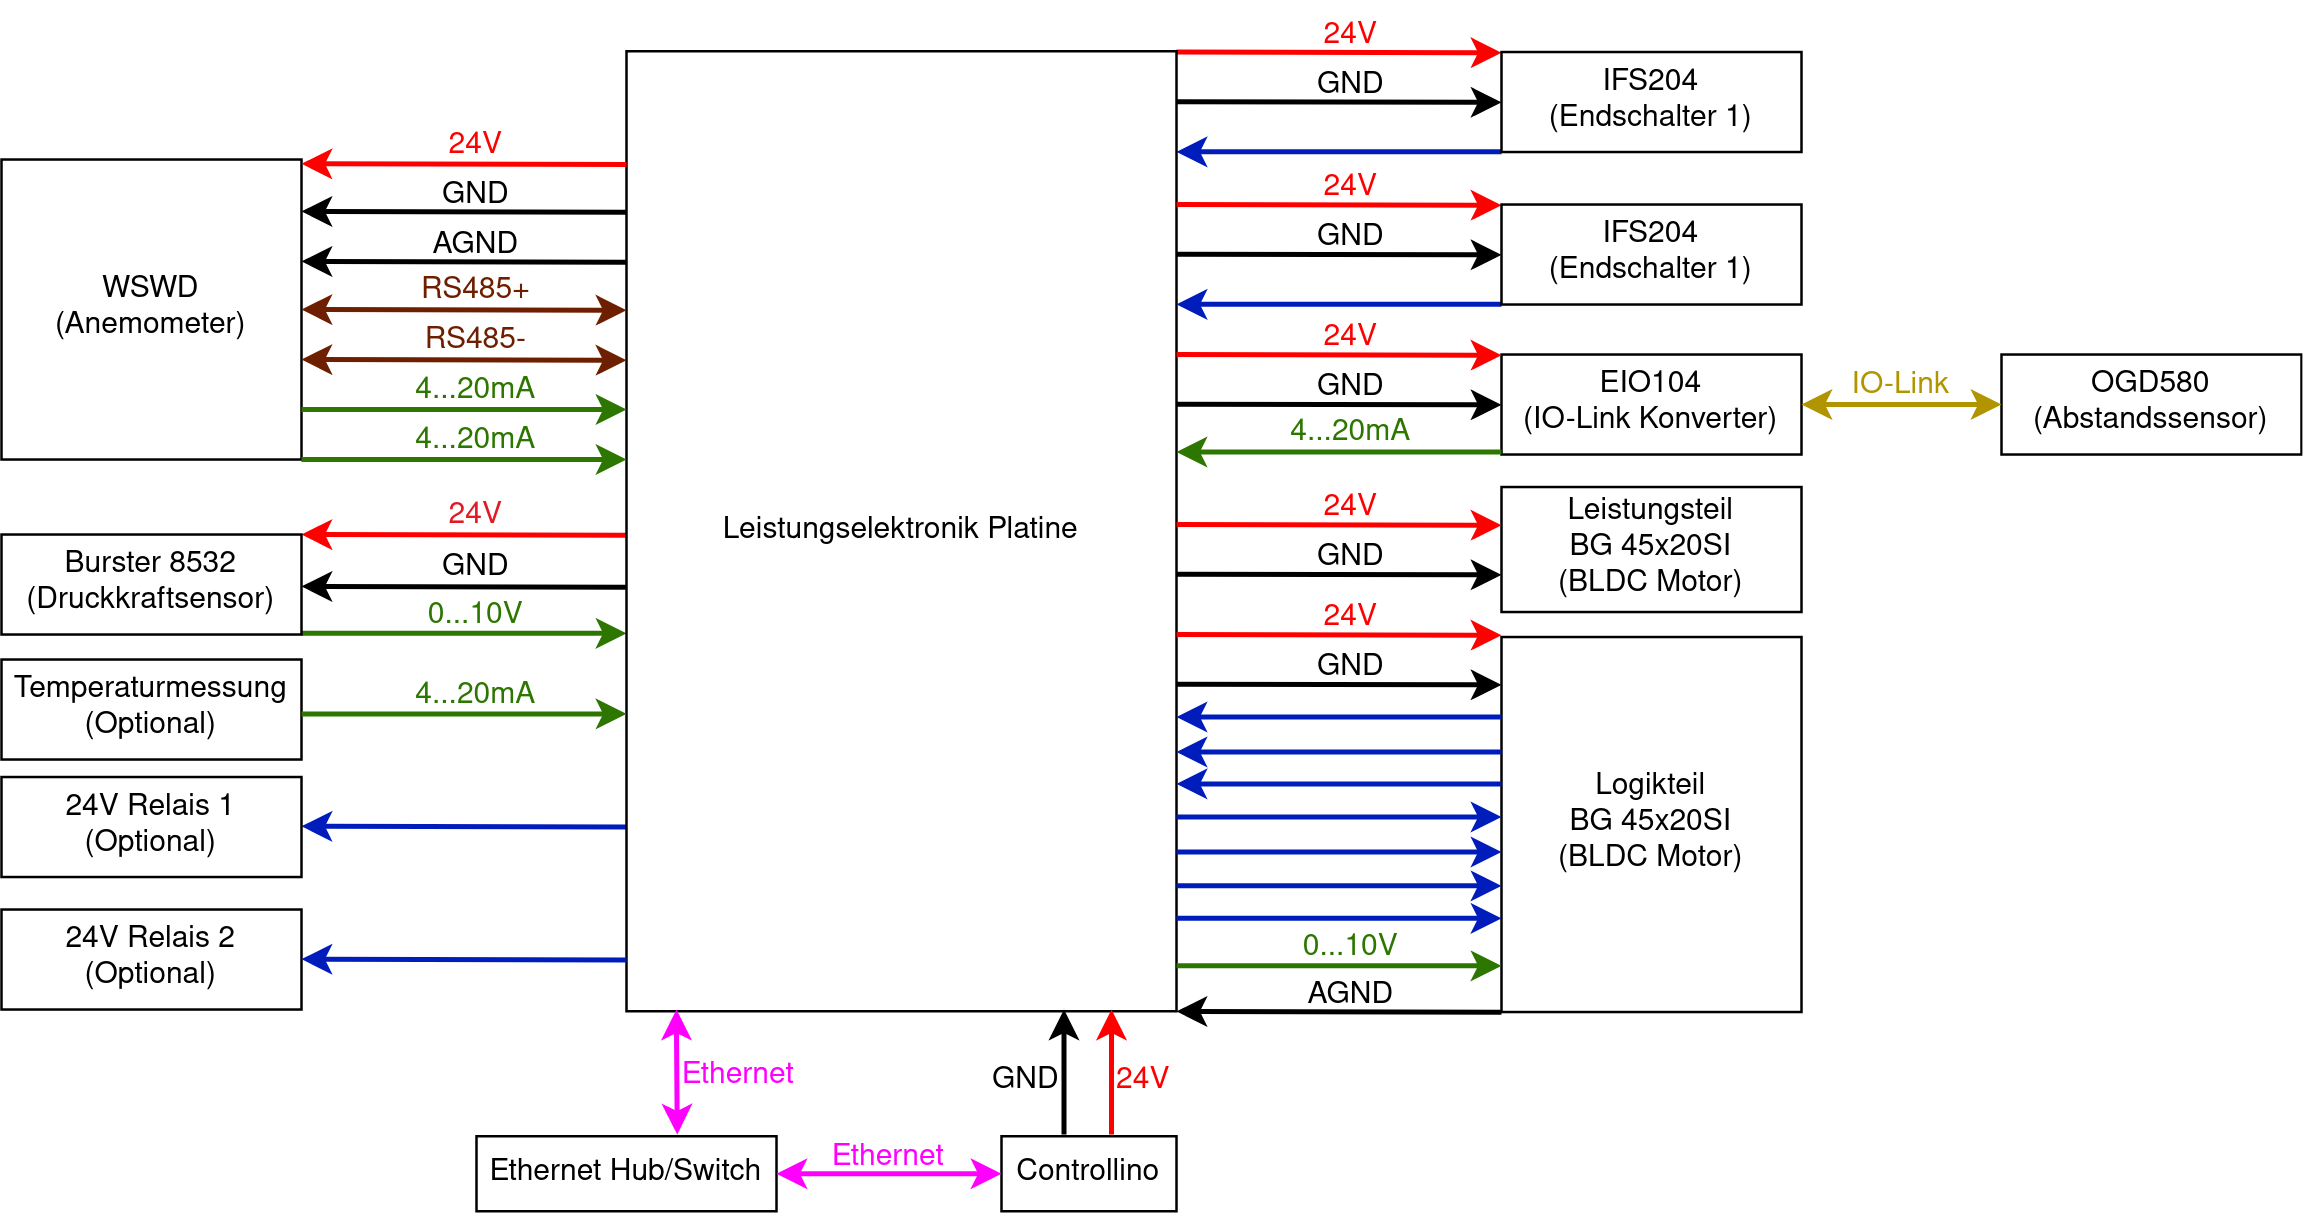
\includegraphics[width=1.0\textwidth]{images/System/Systemaufbau.drawio.png}
	\caption{Blockschaltbild der benötigten Ein- und Ausgänge der Platine}
	\label{fig:System_Aufbau}
\end{figure}
% Please add the following required packages to your document preamble:
% \usepackage{graphicx}
\begin{table}[H]
	\centering
	\resizebox{\textwidth}{!}{%
		\begin{tabular}{|l|lllllllllll|}
			\hline
			\textbf{Element} & \multicolumn{11}{l|}{\textbf{Pinout}} \\ \hline
			\textbf{Endschalter 1} & \multicolumn{1}{l|}{24V} & \multicolumn{1}{l|}{GND} & \multicolumn{1}{l|}{OUT} & \multicolumn{8}{l|}{} \\ \hline
			\textbf{Endschalter 2} & \multicolumn{1}{l|}{24V} & \multicolumn{1}{l|}{GND} & \multicolumn{1}{l|}{OUT} & \multicolumn{8}{l|}{} \\ \hline
			\textbf{Abstandssensor} & \multicolumn{1}{l|}{24V} & \multicolumn{1}{l|}{GND} & \multicolumn{1}{l|}{IO-Link} & \multicolumn{8}{l|}{} \\ \hline
			\textbf{IO-Link Konveter} & \multicolumn{1}{l|}{24V} & \multicolumn{1}{l|}{GND} & \multicolumn{1}{l|}{AOUT} & \multicolumn{8}{l|}{} \\ \hline
			\textbf{Anemometer} & \multicolumn{1}{l|}{24V} & \multicolumn{1}{l|}{GND} & \multicolumn{1}{l|}{AOUT} & \multicolumn{1}{l|}{AOUT} & \multicolumn{1}{l|}{AGND} & \multicolumn{1}{l|}{RS485+} & \multicolumn{1}{l|}{RS485-} & \multicolumn{4}{l|}{} \\ \hline
			\textbf{Druckkraftsensor} & \multicolumn{1}{l|}{24V} & \multicolumn{1}{l|}{GND} & \multicolumn{1}{l|}{AOUT} & \multicolumn{1}{l|}{AGND} & \multicolumn{7}{l|}{} \\ \hline
			\textbf{Motor Leistung} & \multicolumn{1}{l|}{24V} & \multicolumn{1}{l|}{GND} & \multicolumn{9}{l|}{} \\ \hline
			\textbf{Motor Logik} & \multicolumn{1}{l|}{24V} & \multicolumn{1}{l|}{GND} & \multicolumn{1}{l|}{IN0} & \multicolumn{1}{l|}{IN1} & \multicolumn{1}{l|}{IN2} & \multicolumn{1}{l|}{IN3} & \multicolumn{1}{l|}{AIN} & \multicolumn{1}{l|}{AGND} & \multicolumn{1}{l|}{OUT1} & \multicolumn{1}{l|}{OUT2} & OUT3 \\ \hline
			\textbf{Externes Relais 1} & \multicolumn{1}{l|}{OUT} & \multicolumn{1}{l|}{GND} & \multicolumn{9}{l|}{} \\ \hline
			\textbf{Externes Relais 2} & \multicolumn{1}{l|}{OUT} & \multicolumn{1}{l|}{GND} & \multicolumn{9}{l|}{} \\
			\hline
			\textbf{Temperatur Sensor} & \multicolumn{1}{l|}{AOUT} & \multicolumn{10}{l|}{} \\ \hline
			\textbf{Controllino} & \multicolumn{1}{l|}{Ethernet} & \multicolumn{10}{l|}{} \\ \hline
		\end{tabular}%
	}
	\caption{Übersicht Stromversorgung und Schnittstellen der externen Elemente}
	\label{tab:uebersicht-externe-elemente}
\end{table}
\subsection{Auswahl der Platinen Bauteile}
Da nun klar ist welche Anforderungen durch die anzuschließenden Geräte bestehen, kann auf Basis dieser nun weiterverfahren werden. Dabei soll im folgenden ein geeigneter Mikrocontroller, sowie die nötigen Platinenkomponenten ausgewählt werden, um mit den Sensoren und Aktoren zu kommunizieren und diese mit Strom zu versorgen.
\subsubsection{Mikrocontroller}
Die Auswahl des Mikrocontrollers wurde auf der Basis folgender Kriterien beschlossen:
\begin{itemize}
	\item Benötigte Inputs und Outputs
	\item Softwaresupport 
	\item Entwicklung
	\item Verfügbarkeit
\end{itemize}
Dabei gab es die Option den Chip als einzelnes Element direkt auf die selbst erstellte Platine einzubetten oder ein Entwicklungsboard als Basis zu nutzen und eine Erweiterungsplatine dafür zu nutzen. Es wurde sich dabei für ein Entwicklungsboard entschieden um bereits parallel zum Hardwaredesign eine geeignete Software zu entwickeln und diese bereits mit einem Prototypischen Aufbau zu testen (Vielleicht noch erwähnen, probleme bei vorheriger Gruppe). Dies bietet ebenfalls den Vorteil, das beim zerstören des Chips ein schneller Ersatz angebracht werden kann und auch bereits ein Formfaktor vorgegeben ist. Auch kann durch den bereits angebrachten Debugger, schneller neue Software getestet und aufgespielt werden. Ebenfalls besitzen viele Entwicklungsboards bereits einen Ethernetport der sowieso benötigt wird.\\

\noindent Durch die oben genannten Kriterien und die Entscheidung ein Entwicklerboard zu benutzen viel die Wahl auf das STM32 NUCLEO F439zi Board. Diese waren bereits an der HTWG Konstanz Verfügbar, sind durch den Softwaresupport von ST und ihrer eigenen Entwicklungsumgebung einfach zu Programmieren und Aufzusetzen. Außerdem bieten ihre Entwicklungsboards einen abbrechbaren Debugger und das Board kann damit auch außerhalb der Entwicklungsphase eingesetzt werden.
\subsubsection{Relais}
Um das auslösen eines Endschalters an den Mikrocontroller weiterzugeben, werden zwei 24V Relais benötigt die bei der Aktivierung der Spule ein 3,3V Signal an den Eingang des Mikrocontrollers weitergeben. Gleichzeitig soll durch die Relais der Eingang 1 oder 2 des Motors auf Null gesetzt. Diese geben die Drehrichtung an und stoppen den Motor sobald beide auf Null gesetzt sind. Da dieses System unabhängig von der Software des Mikrocontrollers agiert, sollen diese gleichzeitig als Ausfallsichere Aktoren dienen. Hierfür wurden die Omron G6S-2F 24DC Relais ausgesucht. Diese besitzen zwei Schaltbare Ausgänge und haben gleichzeitig einen kompakten Formfaktor.
\subsubsection{Optokoppler}
Um die restlichen 24V Aus- und Eingänge zu steueren oder auszulesen, kommen Optokoppler zum Einsatz. Diese isolieren ähnlich zu Relais den 24V und 3,3V Schaltkreis. Dabei werden insgesamt 9 benötigt um die digitalen Ein und Ausgänge des Motors und die beiden externen Relais zu schalten. Da es sich beim Ausgang 3? des Motors um ein Pulsierendes Signal zur Ermittelung der Drehgeschwindigkeit des Motors handelt wurde auf eine schnelle Schaltzeit der Optokoppler geachtet. Zusätzlich sollte wie bei den Relais wieder ein kleiner Formfaktor vorliegen. Hierfür wurden die LTV-817S ausgesucht. Diese haben mit einer Typischen Schaltzeit von 3-18$\mu$s eine ausreichend Schelle Schaltzeit und ihr kleiner Formfaktor lässt sie gut auf der Platine unterbringen.
\subsubsection{RS485 zu UART Konverter}
Um das Anemometer über die RS485 Schnittstelle zu konfigurieren und Daten abzufragen wird ein zusätzlicher Baustein benötigt. Dieser Konvertiert das differenzielle RS485 Signal zu einem nicht differenziellen \ac{UART} Signal, das der Mikrocontroller untertsützt. Hier wurde der MAX3485CSA+CT-ND ausgesucht da dieser mit einer 3,3V Versorgungsspannung betrieben werden kann und mit bis zu 10$\frac{MB}{s}$ Datenübertragen kann.
\subsubsection{FRAM}
Da die neutrale Position des Segels dauerhaft gespeichert werden soll, wird ein nicht flüchtiger Speicherstein benötigt. Dabei ist der \ac{FRAM} einer der billigsten Speichermöglichkeiten für diesen Zweck. Es wurde die geringste Speichergröße gewählt, da die gespeicherten Daten jederzeit, wie bei einem EEPROM Speicher, überschrieben werden könnem. Hier wurde der FM25L16B-GTR gewählt, dieser hat eine Speicher von 16Kbit und ist damit zum Speichern der Positionsdaten mehr als genügend. Da er über eine \ac{SPI} Schnittstelle angesteuert wird, sind die Schreib- und Lesegeschwindigkeiten sehr schnell. Ebenfalls ist die Lebenserwartung von 85Jahren des Speichers bei 20Mhz Taktfrquenz mehr als ausreichend.
\subsubsection{Operations Verstärker}
Um die Drehzahl des Motors vorgeben zu können, wird ein Analoges Signal im Bereich von 0-10V benötigt. Da der \ac{DAC} des Mikrocontroller bei einer Versorgungsspannung von 5V maximal ein Analoges Signal von 3,3V Ausgeben kann \cite{STM32}, wird ein Operationsverstärker benötigt. Dieser soll mit einem 24V Offset Spannung das Ausgangssignal auf bis zu 10V skalieren. Hier gab es bis auf die maximal Spannung keine großen Anforderungen an den Operationsverstärker und es wurde der weitvebreitet LM2904QS ausgewählt.
\subsubsection{DC/DC-Wandler}
Um alle Komponenten zu versorgen Bedarf es insgesamt 3 verschieden Spannungspotenzialen: 24V, 5V und 3,3V. Um dies zu erreichen sollen alle externen Komponenten direkt mit den 24V versorgt werden. Der Mikrocontroller soll mit den 5V versorgt werden, da er somit auch ohne Debugger Erweiterung genutzt werden kann \cite{STM32}. Hierfür wird ein Step Down Konverter genutzt der die 24V Versorgungsspannung auf 5V herunterbricht. Die 5V sollen daraufhin auf weitere 3,3V mit einem Festspannungsregler heruntergebrochen werden, um die sonstigen Bauteile mit dieser zu Versorgen. Bei der Auswahl wurde darauf geachtet, dass der Konverter einen ausreichenden Strom zu Verfügung stellt ohne dabei dauerhaft unter Vollast zu laufen. Da der Mikrocontroller bis zu 250mA verbraucht musste darauf geachtet werden das der Konverter mehr als diesen Strom zu Verfügung stellt. Es wurde davon Ausgegangen das die restlichen Bauteile nicht mehr als zusätzliche 250mA verbrauchen. Aus diesem Grund wurde der R-78E5.0-0.5 Ausgewählt. Dieser stell bis zu 0,5A an Strom zu Verfügung und kann bei Bedarf mit der 1A Version ausgetauscht werden. Als Festspannungsregler wurde der LM3940IMP-3.3 gewählt. Dieser kann Eingangsspannung von bis zu 7.5V in eine Ausgangsspannung von 3,3V umwandeln und hat dabei einen durchsatz Strom von bis zu 1A. Damit genügt er den Anforderungen.
\subsubsection{Strom Sensor}
Zur Überwachung des Motor Stroms kommt ein Hallstromsensor zum Einsatz. Dieser ist im Gegensatz zu einem Resistiven Sensor genauer und isoliert den 24V und 3,3V Schaltkreis. Er sollte in der Lage sein den maximal zulässigen Motorstrom messen zu können. Da die meisten Hall Sensoren deutlich mehr als diesen messen können wurde sich für den TMCS1101A3BQDRQ1 entschieden. Dieser kann einen maximalen Strom von $\pm$11,25A messen. Der gemessen Strom wird als analoges 0-3,3V Signal ausgegeben.
\subsubsection{Konnektoren}
Die externen Komponenten sollen über Schraubklemmen direkt an die Platine angeschlossen werden. Je nach Querschnitt der Kabel wurde ein größeres oder kleineres Rastermaß gewählt um Platz auf der Platine einzusparen. Dabei wurde als Standard Rastermaß 2,54mm gewählt und für die Kabel mit größerem Durchschnitt ein 3,5mm Rastermaß.
\subsubsection{Analoge Eingänge}
Um die Analogen Ausgänge des Abstandsensors und des Anemometers auszulesen wird das 4-20mA Stromsignal über einen Widerstand zu einem 0-3V Spannungssignal gewandelt das mit dem \ac{ADC} des Microcontrollers gelesen werden kann.
\subsection{Gehäusebauteile}
Um die Platine die sich später in der Kuppel befinden soll, vor z.B Staub und Wasser zu schützen soll diese in einem Gehäuse untegebracht werden. Das Gehäuse sollte vorallem im Innenraum genug Platz bieten um Kabel an der Platine zu befestigen, eine Möglichkeit bieten die Platine darin zu befestigen und genug Platz auf der Oberfläche bieten um die Bedienoberfläche und die unterschiedlichen Kabel Durchführungen zu positionieren. Dabei wurde das Hammond Manufacturing RP1465 gewählt. 
\begin{figure}[H]
	\centering
	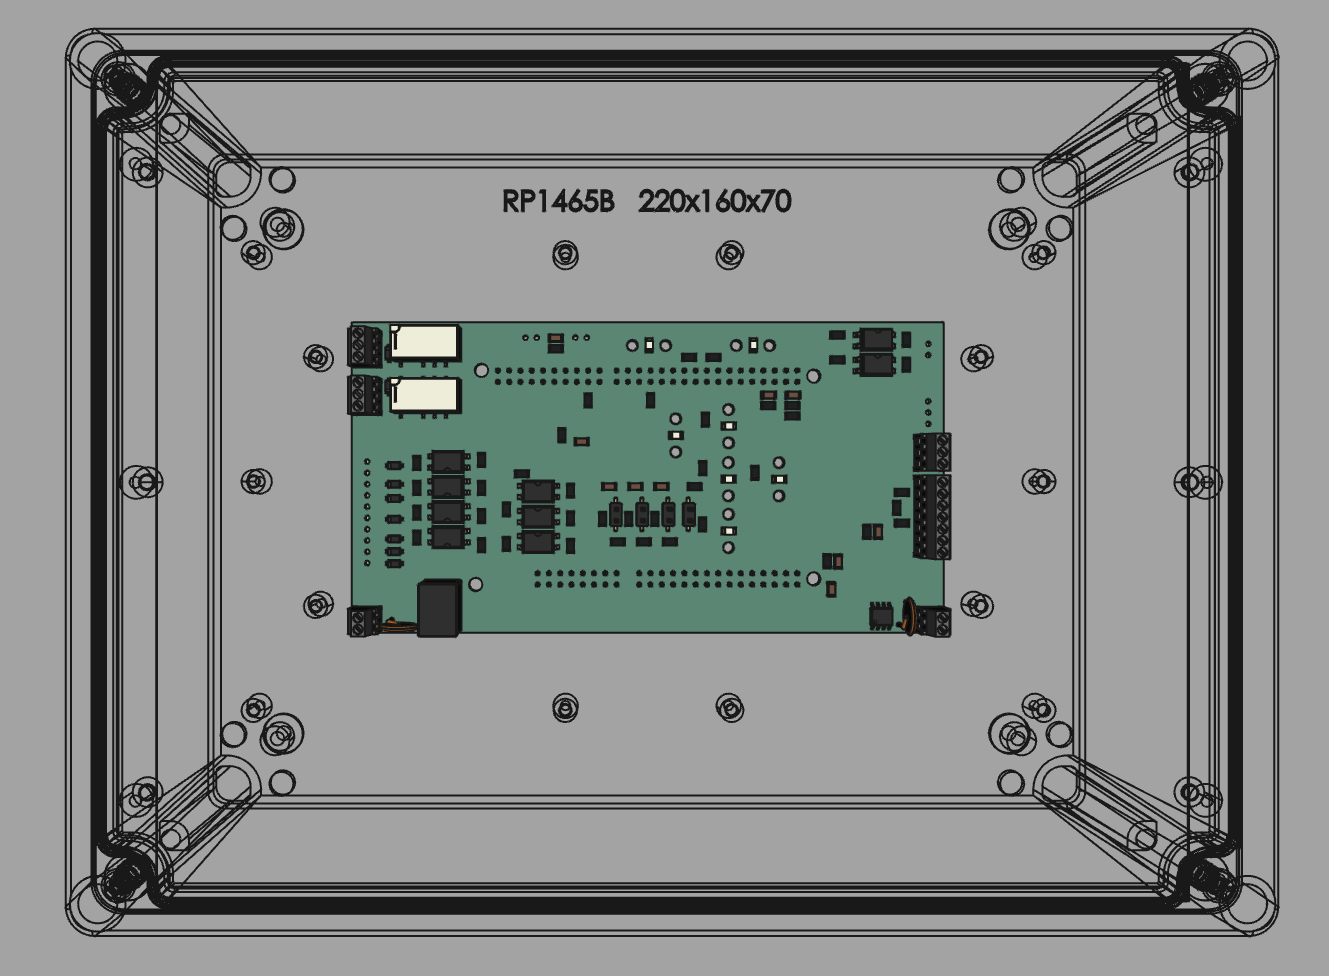
\includegraphics[width=0.8\textwidth]{images/Hardware/Platine_in_gehause.PNG}
	\caption{3D Modell der Platine innerhalb des Gehäuses}
	\label{fig:Gehaues_und_Platine}
\end{figure}
\noindent Dieses bietet genug Platz für die Platine und alle Kabeldurchführungen wie gut in \autoref{fig:Gehaues_und_Platine} zusehen ist. Es bietet ebenfalls die Möglichkeit einen zweiten Boden einzusetzen auf dem der Mikrocontroller und die Platine mit einer 3D gedruckten Befestigung angeschraubt werden können.\\

\subsubsection{Bedienoberfläche}
\noindent Die Bedienoberfläche besteht aus einer Reihe von Kippschaltern, Knöpfen und LEDs. Diese sind sind in \autoref{fig:Bedienung} dargestellt. Dabei soll die gewünschte Neutrale Position der Linearführung durch einen Kalibrierungsfahrt stattfinden. Dabei kann der Endnutzer über die Trimm und Roll Knöpfe zum gewünschten Mittelpunkt Navigieren und diesen mit dem dritten Knopf speichern. Anschließend kann mittels des Kippschalters in den Automatik Betrieb gewechselt werden in dem das betätigen der Knöpfe ignoriert wird.
Eine Reihe von LEDs gibt Feedback über den aktuellen Zustand der Linearführung. Dabei wird konstant der aktuelle Betriebsmodus durch zwei LEDs angegeben. Ebenfalls wird die Position relativ zur festgelegten neutral Position durch zwei gelbe LEDs angegeben. Eine Störung in der Steuerung oder im Motor wird durch eine rote LED angegeben.\\
Die Knöpfe und Kippschalter sind beide am Gehäuse montiert und sind durch Dichtungsringe Spritzwasser geschützt. Die Kabel werden über Dupont Stecker auf der Platine verbunden. Im Gegensatz dazu sind die LEDs direkt auf der Platine platziert und werden durch flexible Lichtleiter zur Außenseite des Gehäuses geführt.
\begin{figure}[H]
	\centering
	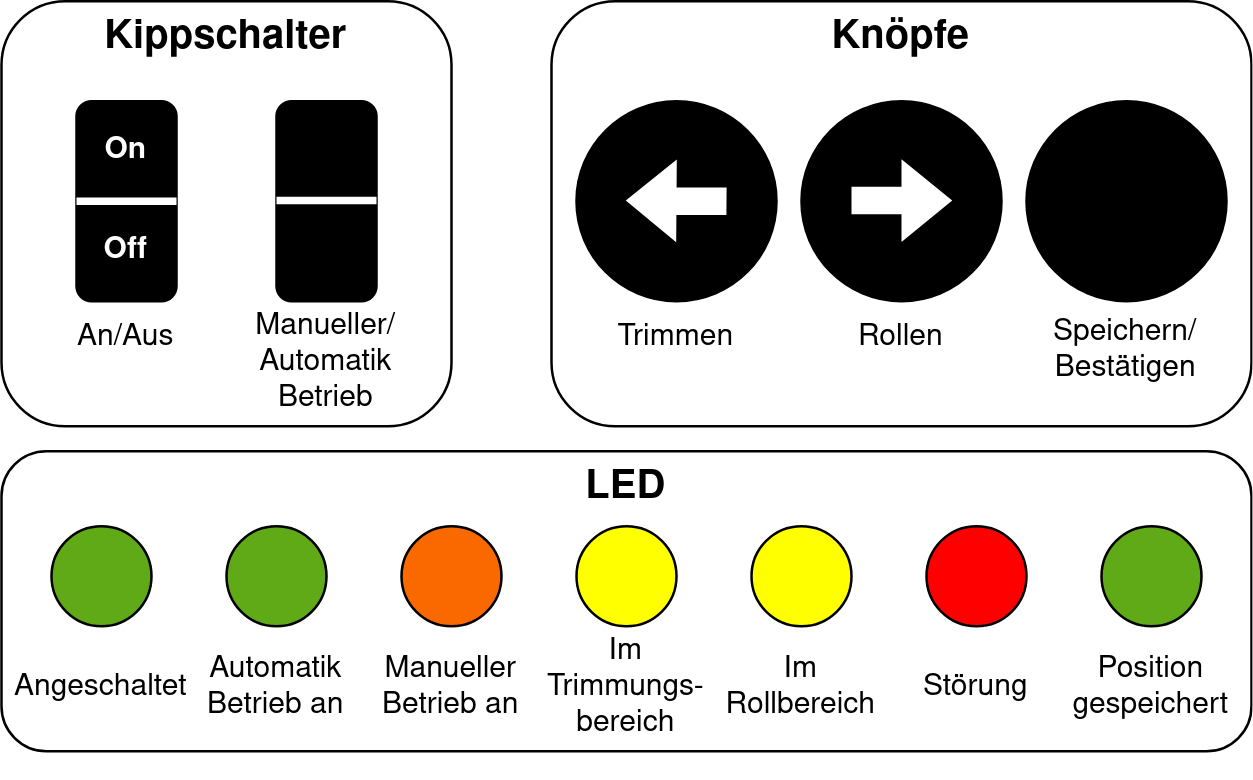
\includegraphics[width=1.0\textwidth]{images/Hardware/Bedienung.drawio.png}
	\caption{HMI der Segel Steuerung}
	\label{fig:Bedienung}
\end{figure}
\subsubsection{Kabelverschaubungen}
Um die benötigten Kabel zu Platine zu führen wurden Kabelverschraubungen in die Seiten des Gehäuses eingelassen. In diese können die Isolierten Kabel eingeführt werden und die Adernkabel an die richtige Position innerhalb des Gehäuses verlegt werden. Die Kabelverschraubungen sorgen ebenfalls für eine Zugentlastung der Kabel an sich.
\subsection{Platinen Schaltplan}
\begin{figure}[H]
	\centering
	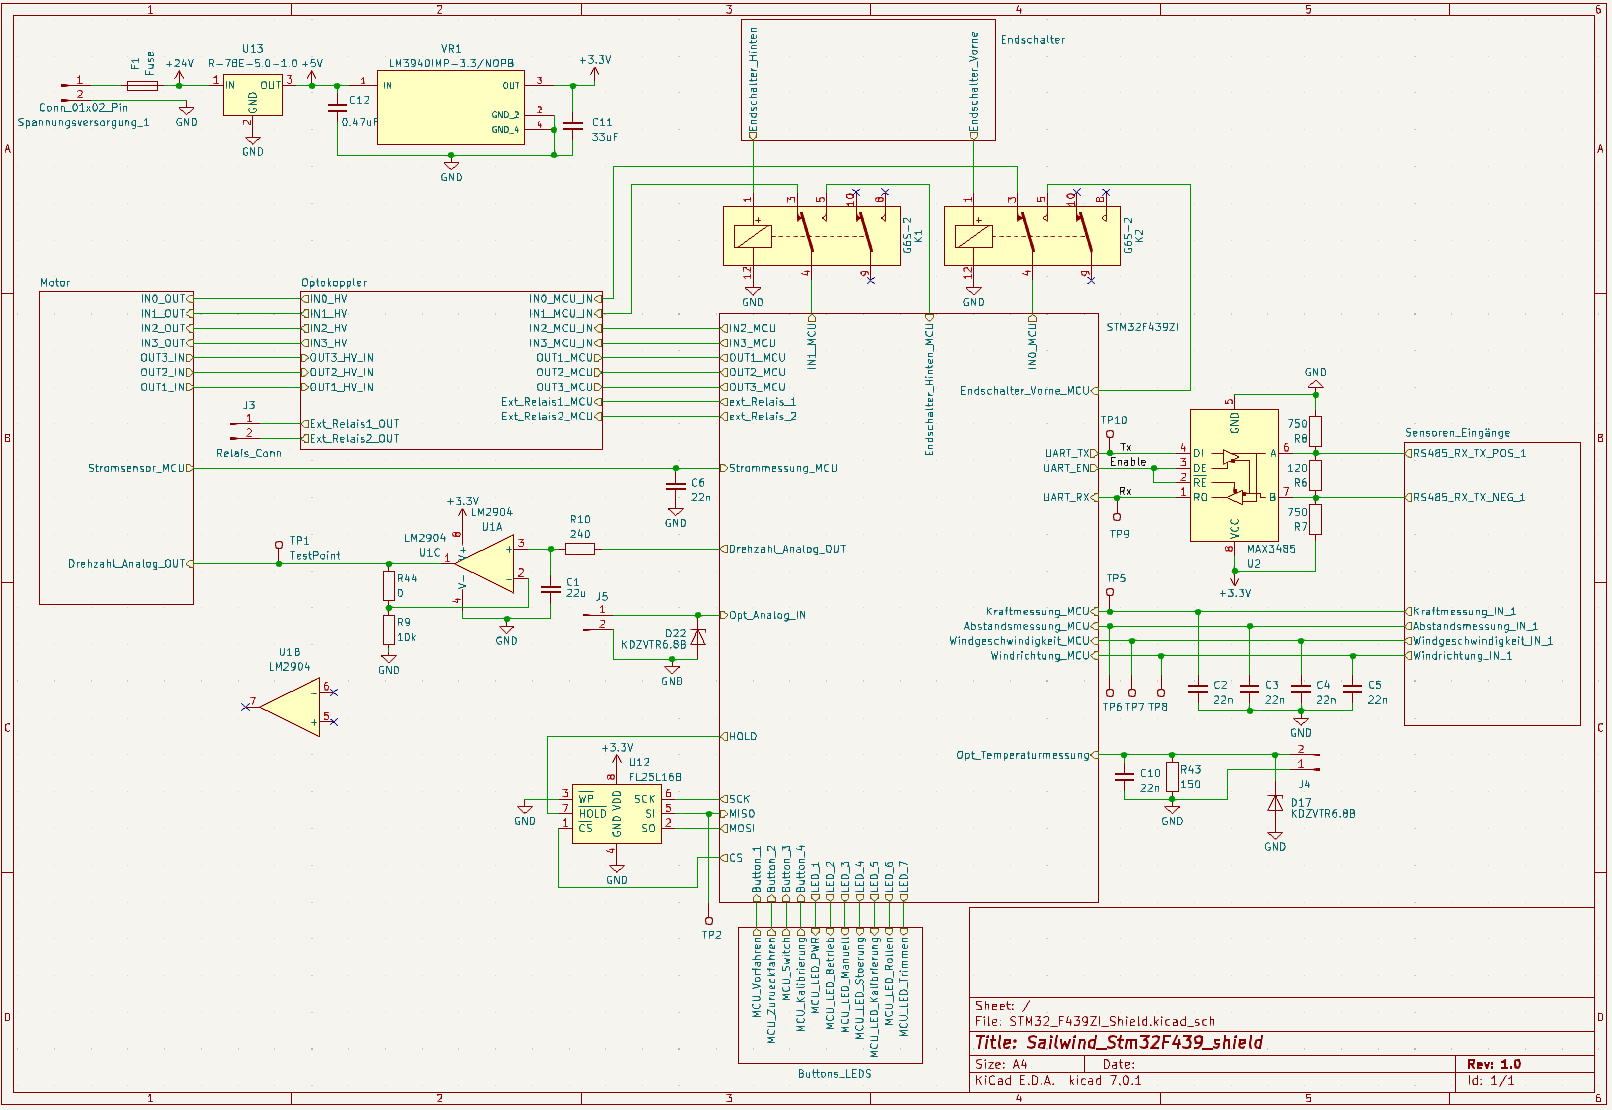
\includegraphics[width=1.0\textwidth]{images/Hardware/Schaltplan_Gesamt.PNG}
	\caption{Gesamtschaltplan der Platine}
	\label{fig:Schaltplan_gesamt}
\end{figure}
Der komplette Schaltplan ist in \autoref{fig:Schaltplan_gesamt} dargestellt und ist ebenfalls im Anhang \autoref{Anhang_Schaltplan} zu finden. Der Schaltplan ist in unterschiedliche Bereiche eingeteilt die die Gruppierung der Komponenten wiedergibt. Dabei ist die STM32 Gruppe zentral Positioniert und alle Bauteile und Komponeten um diese verteilt. Bauteile die nur einfach Verbaut sind wie z.B der FL25L16B \ac{FRAM} (Unten Links) wurden nicht in Gruppen eingeteilt sondern direkt in der Gesamtansicht Positioniert. Oben Links befindet sich die Spannungsversorgung der Platine und die \ac{DC}/DC Wandler. Überhalb des STM32 befinden sich die beiden Relais die an die Endschalter verbunden sind. Links außen befindet sich der \ac{BLDC} Motor der mit dem Operationsverstärker und den Optokoppler verbunden ist. Rechts befinden sich alle Analogen Sensoren, bis auf den Stromsensor. Dort ist ebenfalls der MAX3485 \ac{UART} Konvertierer zu sehen. Unterhalb des Mikrocontrollers befinden sich die Knöpfe und LEDS die das \ac{HMI} bilden. Im folgenden sollen exemplarisch die Schaltungen für diese Gruppen genauer betrachtet werden. Der komplette Schaltplan ist ebenfalls im Anhang hinterlegt.
\subsubsection{STM32F439zi Gruppe}
Die STM32F439zi enthält alle Pins auf denen später die Erweiterungplatine aufsitzt. Hier wurden alle benötigten Pins nach außen geführt.
\subsubsection{Motor Gruppe}
In der Motorgruppe ist neben den Ein- und Ausgängen des BG 45x30 SI auch der Hall Stromsensor abgebildet. Alle digitalen Ein- und Ausgänge auch außerhalb der Motorgruppe sind durch 24V Zener Dioden geschützt die als Überspannungsschutz agieren. Die Spannungsversorgung der Platine und des Motors sind zusätzlich durch Sicherungen vor einem Überstrom geschützt, wie anhand des Stromsensors in \autoref{fig:Motor_gruppe }zu sehen ist.
\begin{figure}[H]
	\centering
	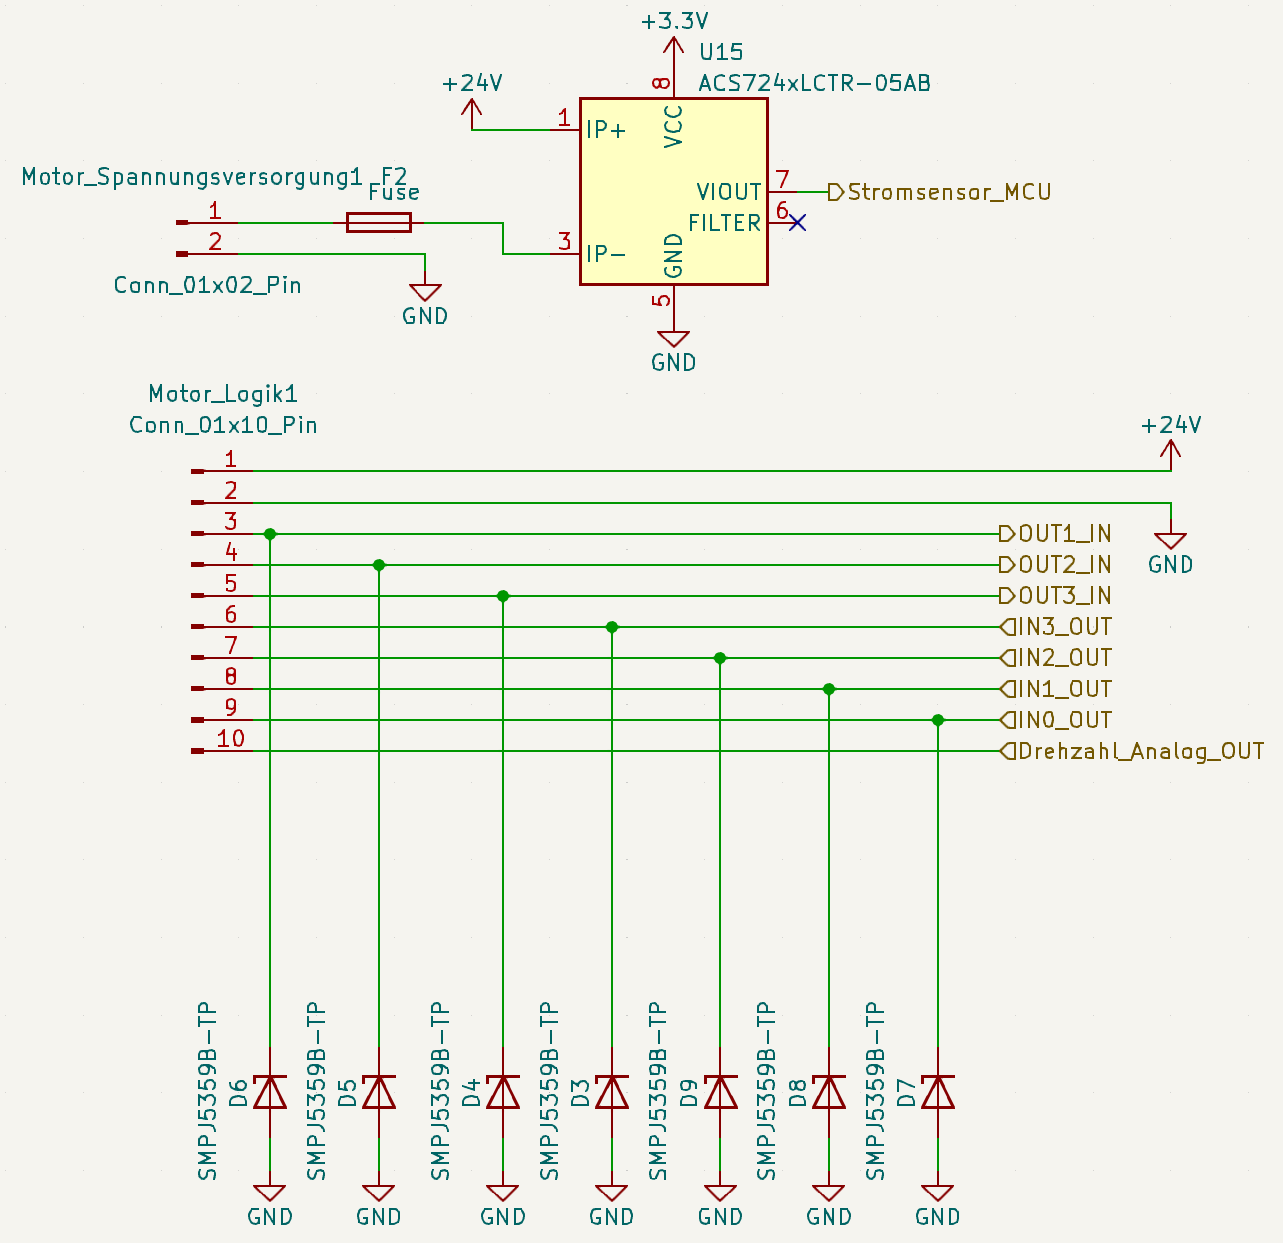
\includegraphics[width=1.0\textwidth]{images/Hardware/Motor_Schaltplan.PNG}
	\caption{Schaltplan der Motorgruppe}
	\label{fig:Motor_gruppe}
\end{figure}

\subsubsection{Optokoppler Gruppe}
\begin{figure}[H]
	\centering
	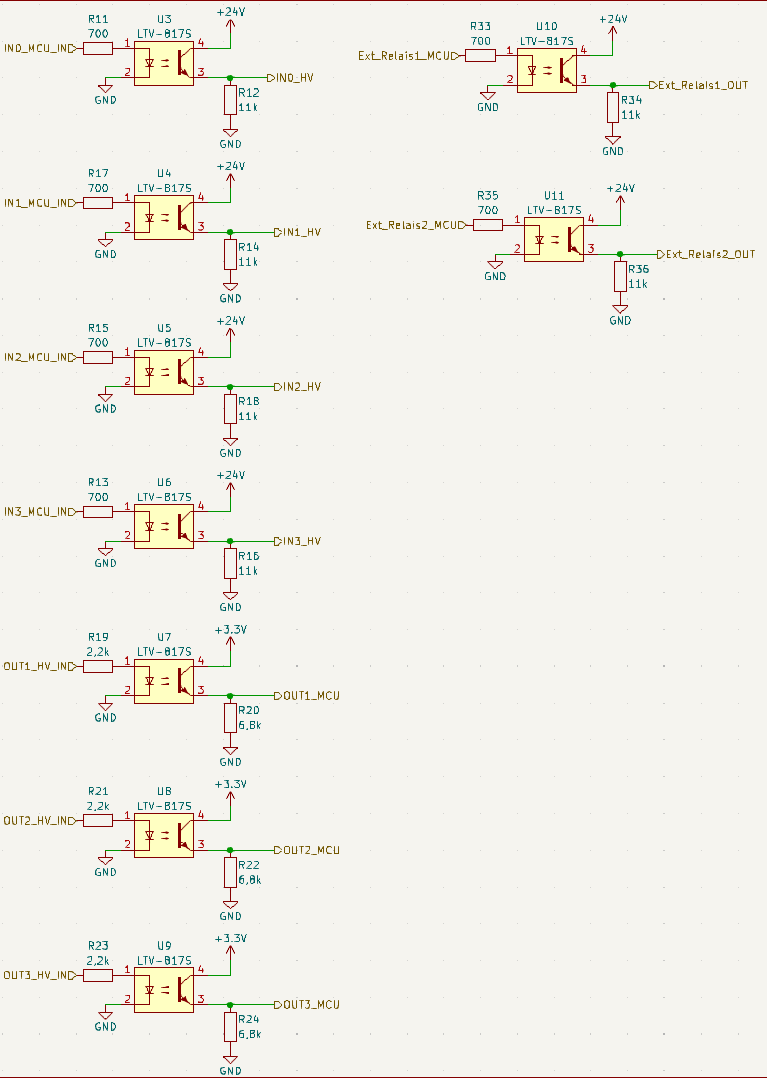
\includegraphics[width=1.0\textwidth]{images/Hardware/Optokoppler_Schaltplan.PNG}
	\caption{Schaltplan der Optokopplergruppe}
	\label{fig:Optokoppler_gruppe}
\end{figure}
Alle Optokopplerschaltungen der Gruppe sind gleich Aufgebaut. Der Eingangswiderstand (links) begrenzt den Strom der in der verbauten Infrarot LED des Optokopplers den Stromfluss auf der Ausgangsseite bestimmt. Ein Pulldown Widerstand auf der Ausgangsseite begrenzt den maximal erlaubten Strom zum Mikrocontroller und setzt den Eingang auf ein festgelegtes Potenzial.
\subsubsection{Sensoren Gruppe}
In der Sensoren Gruppe sind die Analogen Sensoren abgebildet. Hier ist gut zu erkennen wie die Strom Singale in Spannungs Signale von einem Widerstand umgewandelt werden. Für die 4-20mA Signale wurde dabei ein 150$\Omega$ Widerstand gewählt da damit bei einem maximalen Strom von 20mA fast die 3,3V erreicht werden:
\begin{equation}
	U = 20mA\times150\Omega = 3V
\end{equation}
Das Spannungssignal von dem Druckkraftsensor wird durch einen Spannungsteiler ebenfalls auf 0-3V skaliert:
\begin{equation}
	U_{Ausgang} = \frac{10V}{2300\Omega + 1000\Omega}\times1000\Omega = 3,03V
\end{equation}
Um die Analogen Signale stabiler zu halten und niedrige Frequenzen zu entfernen wurden für jedes Analoges Signal ebenfalls Keramik Puffer Kondensatoren mit einer Kapazität 22nF hinzugefügt.
\begin{figure}[H]
	\centering
	\includegraphics[width=1.0\textwidth]{images/Hardware/Sensoren_Eingänge_Schaltplan.PNG}
		\caption{Schaltplan der Buttons und LEDs}
	\label{fig:Sensoren_Gruppe}
\end{figure}
\subsubsection{Buttons und LEDs Gruppe}
Für die Buttons wurde eine Debounce Schaltung integriert, damit das Debouncing nicht über die Software geregelt werden muss. Hierbei wurde ein RC Filter genutzt. Beim drücken des Knopfes wird der Kondensator dabei zuerst entladen was zu einer langsam abfallend Spannung führt. Wird der Knopf losgelassen lädt sich dieser wieder auf. Somit kommt nie ein Sprung innerhalb der Spannung vor. Da die Debounce Zeit der Knöpfe typisch bei 0,1ms liegt wurde von einer Zeitkonstante $\tau$ = 10ms für den RC Filter ausgegangen. Die \ac{LED}s wurden je nach zulässigen Strom mit einem entsprechenden Widerstand versehen.
\begin{figure}[H]
	\centering
	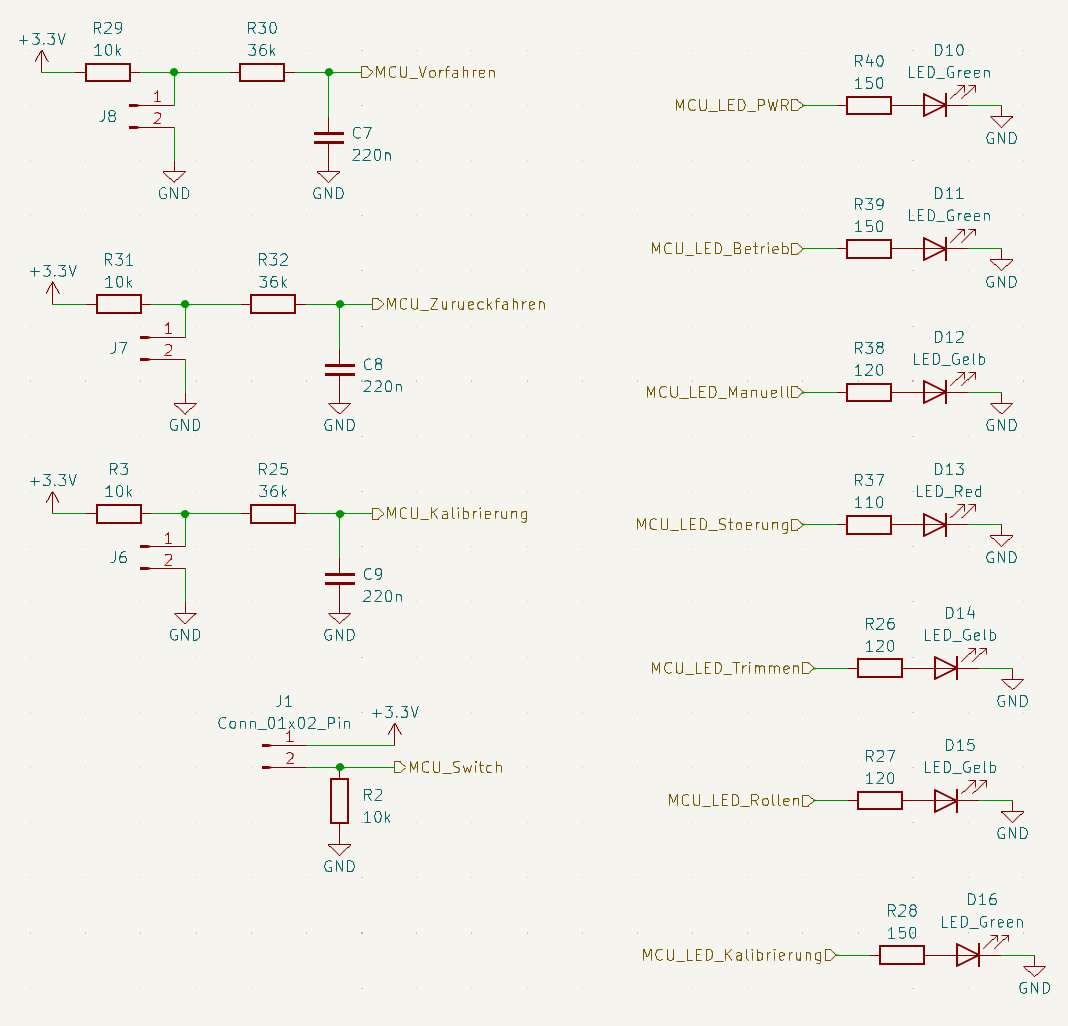
\includegraphics[width=1.0\textwidth]{images/Hardware/LEDS_und_buttons_schaltplan.PNG}
	\caption{Schaltplan der Buttons und LEDs}
	\label{fig:HMI_Gruppe}
\end{figure}
\subsection{\ac{PCB}}
Das fertige PCB ist als 3D Modell in \autoref{fig:PCB_3D} dargestellt. Beim Positionieren der Komponenten wurde daraufgeachtet die 24V Komponenten von den 3,3V Komponenten zu trennen. Aus diesem Grund befinden sich die 24V Komponenten am Rand der Platine während die 3,3V Bauteile mehr im inneren der Platine Positioniert sind. Die Platine sitzt mit vier unterschiedlichen Pin Reihen auf dem Entwicklungsboard auf und führt die Pins auf die Oberseite der Platine. Die dicke der Spuren auf der Platine wurde durch den Strom, die Spannung und Länge bestimmt. Da der Hersteller der Platine vorgegeben hat, das die kleinste Spurbreite 0,2mm sein kann, reichte diese für die meisten Spuren aus. Die Spur über die der Motorstrom fließt ist dabei die einzige breitere, da diese bis zu ca. 4A standhalten muss.
\begin{figure}[H]
	\centering
	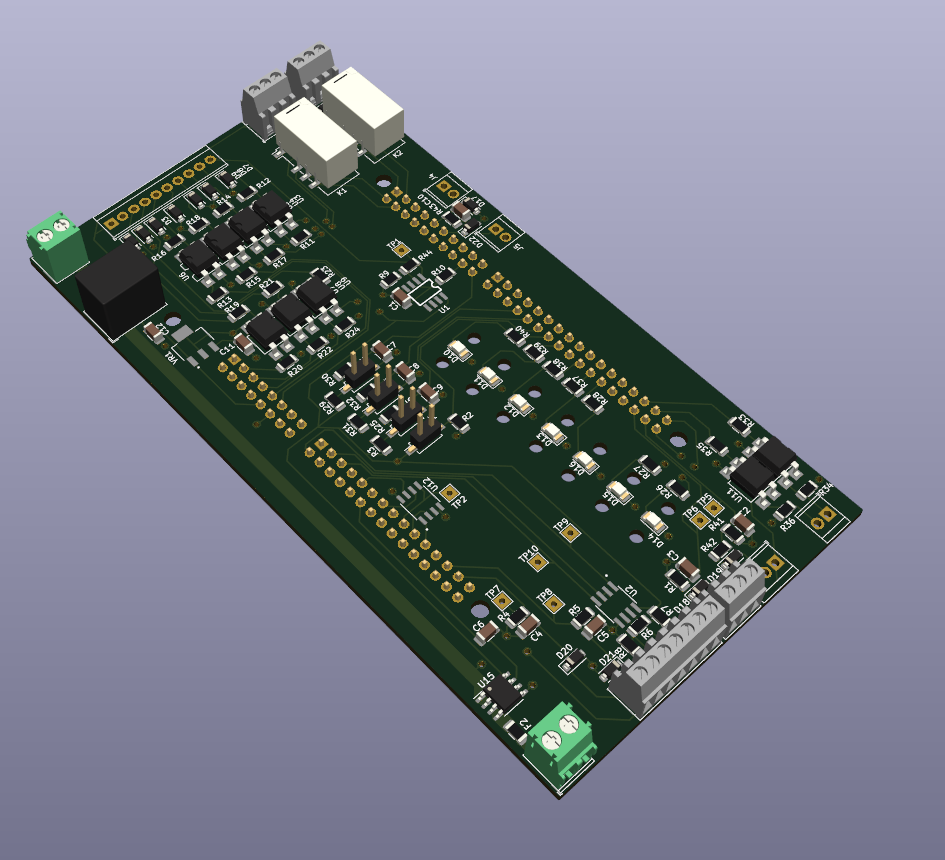
\includegraphics[width=1.0\textwidth]{images/Hardware/Platine_Fertig_3D_ansicht(1).PNG}
	\caption{3D Ansicht des fertigen PCBs}
	\label{fig:PCB_3D}
\end{figure}


\subsection{Probleme}
Während der Nutzung und Bestückung des \ac{PCB}s sind einige Probleme aufgetreten. Diese waren auf das Design oder falsche Berechnungen zurückzuführen. Diese sollen im folgenden erklärt und korrigiert werden.
\subsubsection{Schraubklemmen Löcher}
Der erste Fehler der zu Beginn auffiel, war der Durchmesser der Löcher für die Schraubklemmen. Diese waren zwar groß genug dimensioniert um die Pins Schraubklemmen durchzuführen, aber waren nicht darauf angepasst Nieten einzufügen um die Pins elektrisch mit der Platine zu verbinden. Die Löcher waren ebenfalls zu klein um mit Drähten eine elektrische Verbindung zwischen dem Pin und dem Board herzustellen. Dies führte zu vielen elektrischen Kontakt Problemen und minderte die horizontale Stabilität der Schraubklemmen. Die Kontakt Probleme führten auch zur mangelnden Präzision der Analog Eingänge (siehe \autoref{Mangelnde_Präzision}).
\subsubsection{Operationsverstärker}
Der Operationsverstärker war zwar als Verstärkerschaltung richtig konfiguriert, allerdings musste die Verstärkerspannung von 3,3V auf 24V angehoben werden, um die 10V zu erreichen. Zusätzlich wurde der Spannungsteiler am Ausgang des OPVs entfernt und der erste Widerstand gegen einen 0Ohm Widerstand getauscht.
\subsubsection{RS485 Bias Widerstände}
Die RS485 Widerstände wurden anfänglich die empfohlenen Widerstände in der WSWD Dokumentation genutzt. Hier wurde bei einer Versorgungsspannung von 5V ein Busabschlusswiderstand $R_t$ von 120$\Omega$ und zwei Biaswiderstände $R_b$ von 750$\Omega$ empfohlen (vgl.\cite{WSWD} S.21). Dies sorgte allerdings für eine zu große Differenz der beiden Spannungen und der MAX3485 konnte nicht zwischen high und low unterscheiden. Deshalb wurde stattdessen nach der Anleitung des MAX3485 die Differenz zwischen beiden Potenzialen auf 0,2V begrenzt. Hierfür wurde auf die Berechnung in dem von Texas Instruments veröffentlichten Bericht: \glqq{}RS-485 failsafe for an idle bus\grqq{} zurückgegriffen. Hier lässt sich anhand der Formel: 
\begin{equation}
	R_b = (\frac{V_s}{V_{diff }}+1)\times27,8\Omega
\end{equation}
die beiden Bias Widerstände für das RS-485 Netzwerk berechnen. Dabei kam für die Eingesetzten Werte:
\begin{equation}
	R_b = (\frac{3,3V}{0,2V}+1)\times27,8\Omega = 486,5\Omega
\end{equation}
Der nächst kleinere Widerstand der Verfügbaren E24 Reihe wurde dann auf 470$\Omega$ gewählt. Damit konnte daraufhin erfolgreich über RS485 kommuniziert werden.
\subsubsection{FRAM Anschlüsse}
Die SPI Anschlüsse des FRAM Speicher wurden falsch verbunden dabei wurden die \ac{MOSI} und \ac{MISO} Leitung vertauscht und der \ac{WP} Pin auf das Ground Potenzial gelegt. Dies führte dazu, dass der Speicher nicht addressiert werden konnte und er nicht auf gesendete Befehle reagiert hat. Zuerst wurde der \ac{WP} von dem Ground Potenzial entfernt und schwebend gehalten. Durch das Beobachten der Pegel von MISO, MOSI und Clock Leitung konnte daraufhin erkannt werden das diese vertauscht wurden. Die PCB Spur wurde dafür getrennt und die Pins mit Kabeln direkt verbunden.
\subsubsection{Abstandssensor Präzision}
Der Abstandssensor war eine weitere große Problem Quelle. Der Abstandsensor hat eine sehr hohe Präzision erreicht diese allerdings erst nach einer Aufwärmzeit. Diese ist laut Datenblatt erst bei einer Umgebungstemperatur von -10°C notwendig (vgl. \cite{OGD580_Datasheet} S.2). Allerdings wurde im Betrieb festgestellt das bei stillstand das Display des Sensors immer sinkende Werte anzeigt. Um die Ursache dafür zu finden wurden einige Messreihen durchgeführt. Hierbei wurde der Abstand zum Sensor konstant gehalten und in einem Interval von 30s der Spannungswert an einem Messpunkt der Platine mit einem Oszilloskop gemessen. Dies wurde für inkrementierende Außerbetriebszeiten wiederholt. Die Messreihe ist in \autoref{OGD580} dargestellt. Hier ist klar erkennbar das erst nach ca. 1400s oder ca 20-25min. ein gleichbleibender Spannungswert auslesbar ist. Ebenfalls geht hier hervor, dass die Präzision mit der Temperatur des Sensors zusammenhängt, da nach kürzeren Außerbetriebszeiten die Differenz sinkt.
\begin{figure}[H]
	\centering
	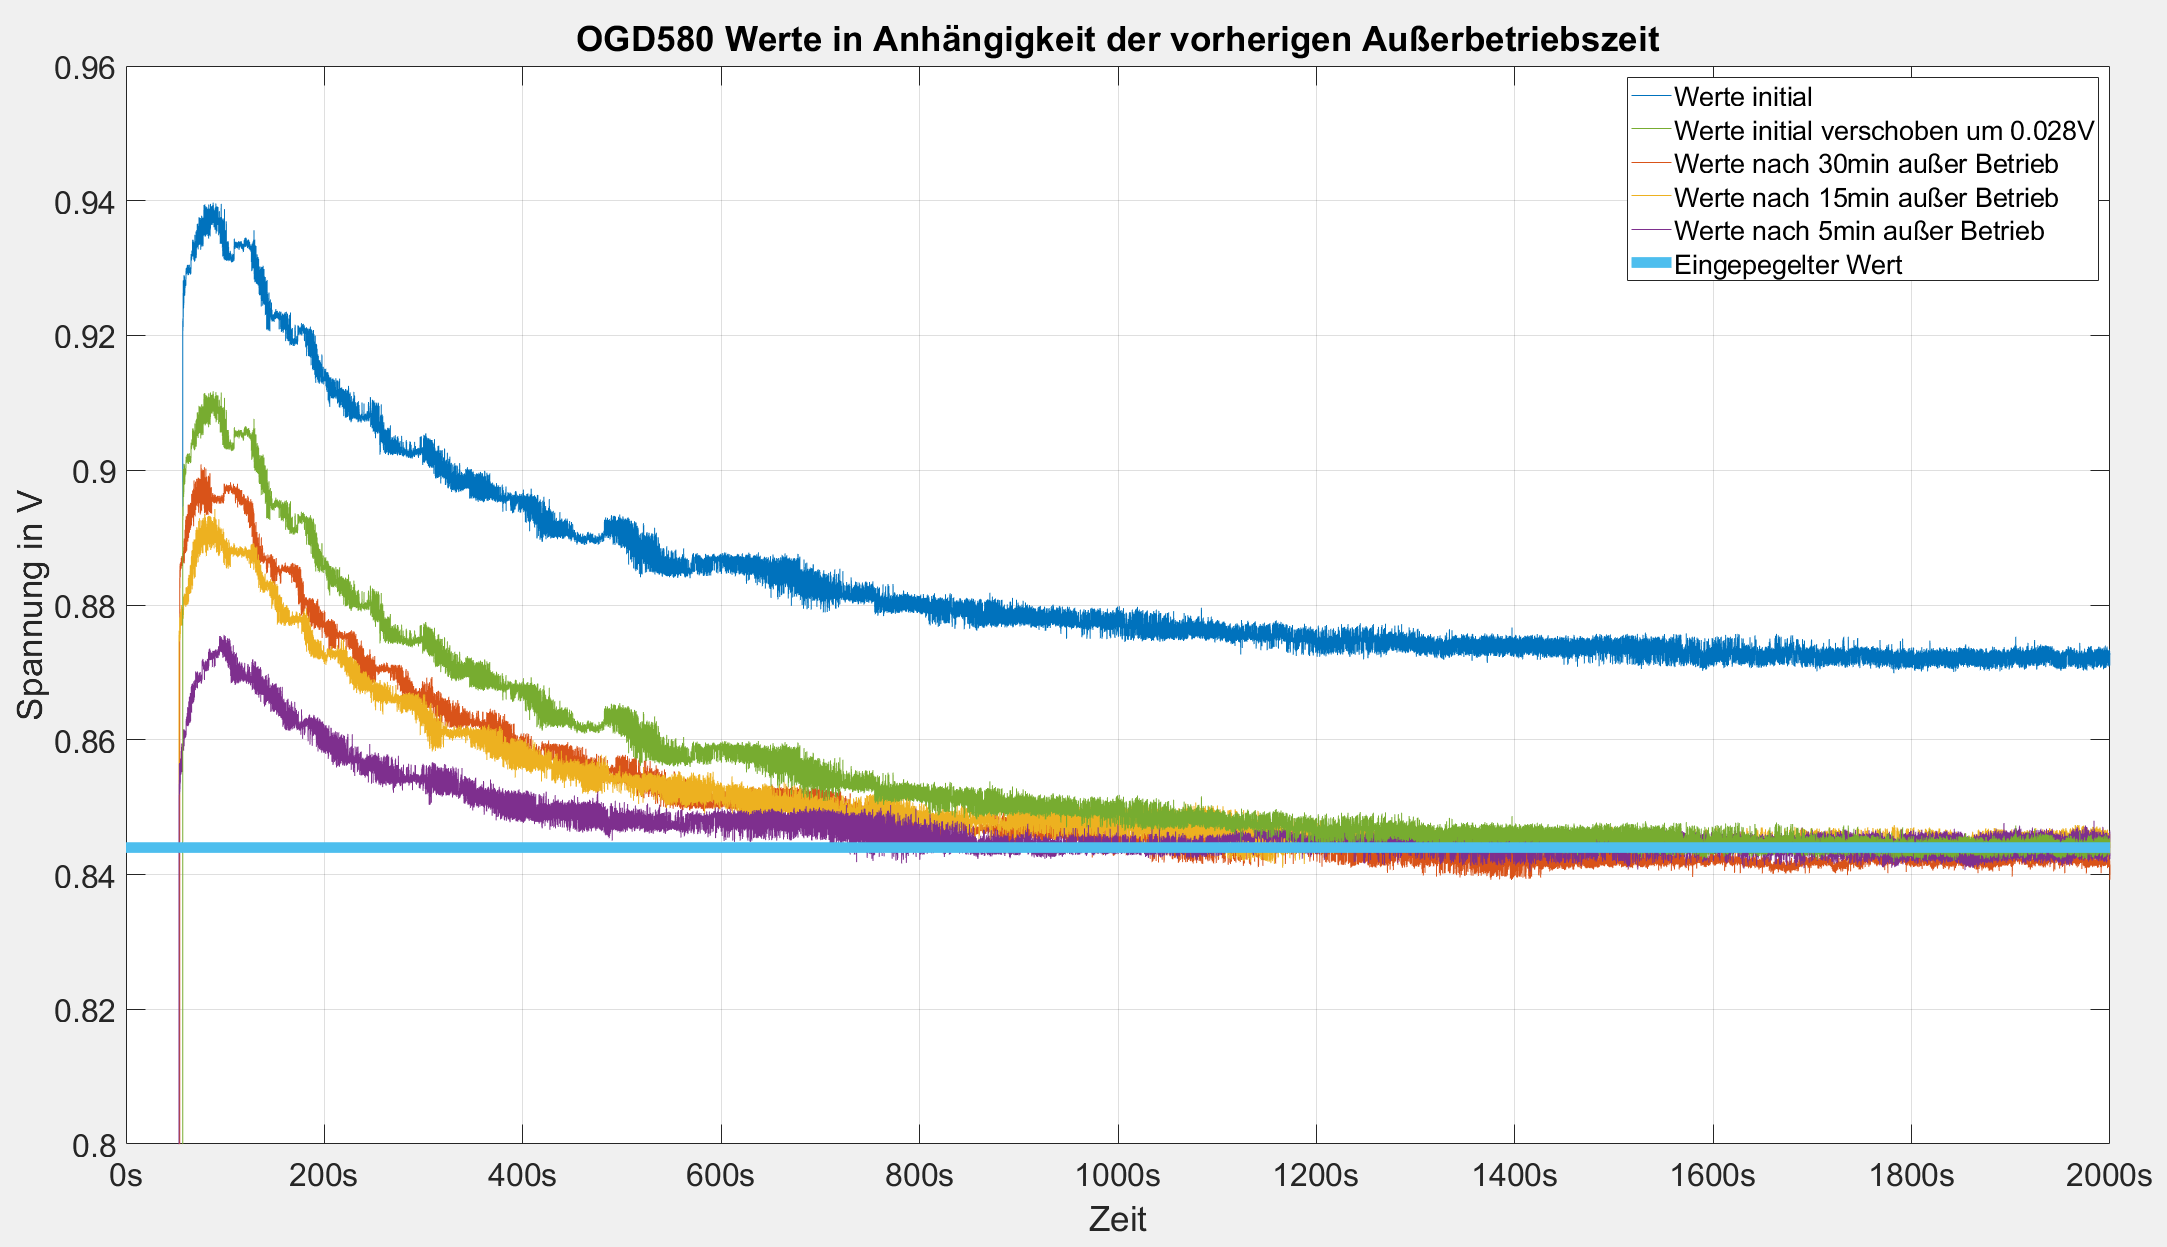
\includegraphics[width=1.0\textwidth]{images/Hardware/Abstandssensor_plot_highres.PNG}
	\caption{Messreihen des ausgelesen Spannungswert bei gleichbleibendem Abstand und steigenden Außerbetriebszeiten}
	\label{fig:Messreihe_Temperatur}
\end{figure}

Das Problem blieb allerdings selbst nach einer Aufwärmzeit von 20min. bestehen. Die Abweichung der ausgelesen Werte über die Messpunkte und den abgelesen Wert am Display lagen teilweise bis zu 25mm auseinander. Um die Ursache des Problems zu finden wurde hier ebenfalls mehrere Messreihen aufgenommen. Hier wurde der Schlitten der Linearführung in 20mm Abständen verschoben. An jedem dieser Punkte wurden folgende Daten notiert:
\begin{itemize}
	\item Abstand zum Sensor gemessen mit einem Meterstab in mm
	\item Angezeigter Abstand auf dem Display des Sensors in mm
	\item Ausgegebener Strom des IO-Link Konverters gemessen mit einem Multimeter in mA
	\item Spannung am Testpunkt der Platine mit einem Oszilloskop in V
\end{itemize}
Dies wurde in 5 Messreihen wiederholt um die Reproduzierbarkeit zu verifizieren. Die aufgezeichneten Daten wurden alle in mm umgerechnet:
\begin{equation}
	L_{Strom} = \frac{L_{max}-L_{min}}{I_{max}-I_{min}}\times(\frac{I_{Position}}{1000}-I_{min}) + L_{min}
\end{equation}
\begin{equation}
	L_{Spannung} = \frac{L_{max}-L_{min}}{I_{max}-I_{min}}\times(\frac{U_{Position}}{153,5\Omega}-I_{min}) + L_{min}
\end{equation}
 und überhalb der mit dem Meterstab gemessen Werte geplotet. Eine dieser Messreihen ist in \autoref{fig:Messreihe_Abstand} dargestellt.
\begin{figure}[H]
	\centering
	\includegraphics[width=1.0\textwidth]{images/Hardware/Messreihe_Präzision.png}
	\caption{Präzision des Abstandssensor anhand verschiedener Messwerte}
	\label{fig:Messreihe_Abstand}
\end{figure}
\noindent Hier ist zu erkennen das der auf dem Display abgelese Abstand mit dem gemessenen Abstand übereinstimmt. Allerdings weichen sowohl der Strom als auch der Spannungswert ab, da die Steigung beider Messreihen nicht gleich zu der des Abstandssensor ist. An diesem ist es möglich eine Skalierung festzulgen. Dabei kann z.B festgelegt werden ab welchem Messwert das Ausgangssignal 4mA/20mA beantragen soll (vgl. \cite{EIO104_Manual}, S.6). Da das Display den korrekten Wert anzeigt, aber ein falscher Strom Wert ausgegeben wird kann davon ausgegangen werden das der Konverter falsch eingestellt ist. Dies konnte im Zuge dieser Arbeit nicht behoben werden, da ein entsprechendes IO-Link Master Gerät nicht verfügbar war.
\subsubsection{Präzision der Analogen Signale}
Neben den Problemen mit den Abstandssensor wurden ebenfalls leicht abweichende Werte in den anderen Analog Signalen festgestellt. Beginnend mit den Strom Signalen, kann der ausgelesene Wert mit der Präzision des Widerstandes zusammenhängen, da diese mit 1\% Genauigkeit immer noch große Temperaturabweichungen aufweisen können. Die schlechten Kontakte tragen ebenfalls zur Ungenauigkeit bei. Speziell bei dem Stromsensor kann es sich ebenfalls um ein positionierungs Problem handeln, da die Verbunden Spuren für optimale Präzision im 45° Winkel zu den Sensor Pins stehen sollten. Um Präzision zu verbessern sollten zusätzlich zu den Präzisieren Widerstände ebenfalls Ferrite eingesetzt werden. Diese verhalten sich ähnlich wie Spulen und filtern hoch Frequente Signale. In Kombination mit den bereits genutzen Kondensatoren sollten diese als LC-Filter funktionieren und einen Bandpass erzeugen.\\
Bilder

        \section{Software}
Die Steuerung der Segel soll durch zwei verteilte Systeme erfolgen, die über eine Ethernet-Verbindung miteinander kommunizieren. Die Idee dahinter ist, die Berechnungen für die Ausrichtung der Segel in Abhängigkeit der Windstärke und -Richtung (Controllino) von der hardwarenahen Verarbeitung der Sensoren und Aktuatoren (STM32) logisch zu trennen. \\

\noindent
Die vorliegende Arbeit konzentriert sich dabei lediglich auf das System der Sensoren und Aktuatoren, welches mit dem STM32 realisiert wurde. Die Aufgabe dieses Systems ist, zunächst die Linearführung zu kalibrieren, damit die aktuelle Position korrekt ermittelt werden kann. Außerdem soll über die Buttons am Gehäuse und zusätzlich über einen Webserver eine manuelle Steuerung ermöglicht werden. Während des Automatikbetriebs geschieht ein regelmäßiger Austausch aller relevanter Daten über eine REST basierte Schnittstelle. Dies beinhaltet u.A. die Information über aktuelle Windbedingung, Position der Segel, eventuelle Fehlerzustände (z.B. Motorfehler oder Überstrom) und daraus resultierende Befehle zur Anpassung der Segelstellung.
Für die Implementierung wurde die Software in komponentenorientierte Module eingeteilt:
\begin{figure}[H]
	\centering
	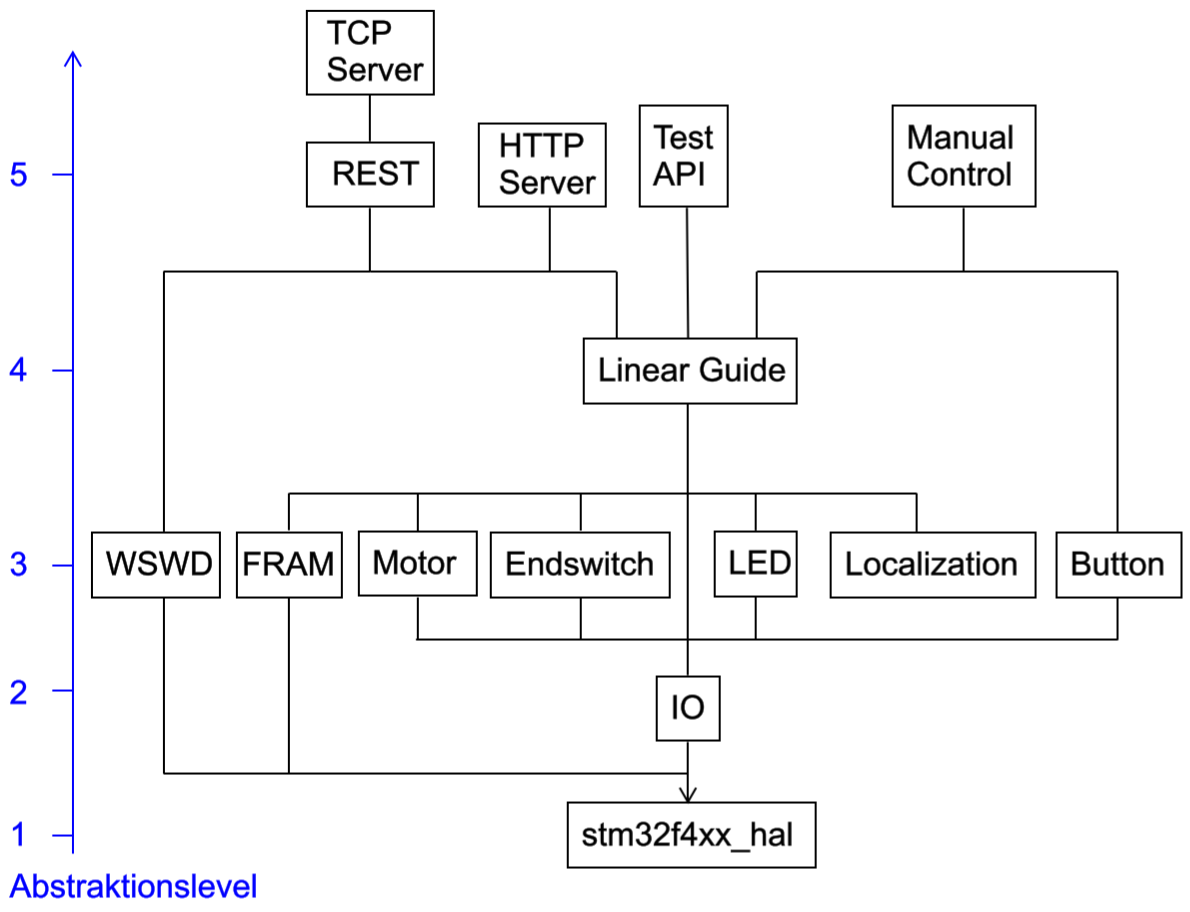
\includegraphics[width=0.6\linewidth]{images/Software/Modulestructure.png}
	\caption{Software Modulstruktur}
	\label{fig:modulestructure}
\end{figure}
\noindent
\autoref{fig:modulestructure} zeigt abwärtsgerichtet, wie die einzelnen Module aufeinander zugreifen. Auf unterster Abstraktionsebene laufen jegliche Operationen über die Standardbibliothek des Mikrocontrollers \verb|stm32f4xx\_hal|. Darüber liefert das \verb|IO|-Modul ein Set aus Hilfsfunktionen und -Strukturen für den allgemeinen Zugriff auf die GPIO-Pins und zum Auslesen analoger Messwerte der einzelnen Sensoren.\\

\noindent
Ebene drei umfasst hauptsächlich Module, welche alle relevanten Funktionalitäten der physischen Teilkomponenten des Systems implementieren, wie z.B. das Anemometer \verb|WSWD| oder der \verb|Motor|. Einige davon greifen dabei auf das \verb|IO|-Modul zu, wobei der allgemeine GPIO-Zugriff von einer spezifischen Funktion eingekapselt wird, wie z.B. das Einschalten einer LED im Falle des \verb|LED|-Moduls. Eine Ausnahme ist das \verb|Localization|-Modul, welches keine physische Komponente darstellt, sondern einige Hilfsfunktionen zur Kalibrierung und Positionsberechnung bereitstellt.\\

\noindent
Während die Module bis Ebene drei überwiegend allgemeingültig entworfen sind, enthält das \verb|Linear Guide|-Modul anwendungsspezifische Funktionen. Als zentrales Element bildet dieses ein High-Level Interface zur Verwendung der Teilkomponenten \verb|FRAM|, \verb|Motor|, \verb|Endswitch|, \verb|LED|, \verb|Localization| und \verb|IO|. \\

\noindent
Die Module der obersten Abstraktionsebene bilden die direkten Schnittstellen zur Außenwelt. Das \verb|Manual Control|-Modul ermöglicht die manuelle Steuerung der Linearführung über die User-Buttons am Gehäuse und insbesondere die Umsetzung des Kalibrierungsprozesses. Auf der anderen Seite kann das System auch durch einen HTTP Webserver überwacht und gesteuert werden. Außerdem werden im \verb|REST|-Modul die Anfragen des Controllinos über die \verb|TCP Server|-Verbindung verarbeitet, wie bereits oben erwähnt. Zuletzt wurde ein \verb|Test|-Modul implementiert, dass die Funktionalitäten der Module auf Ebene drei verifiziert. Dazu wurde ein einfaches Batch-Skript geschrieben, das die einzelnen Testcases auflistet und die Auswahl über UART an den  Mikrocontroller sendet, sodass im \verb|Test|-Modul eine entsprechende Funktion ausgeführt wird. In den nachfolgenden Abschnitten wird genauer auf einige Module eingegangen, beginnend mit dem untersten Abstraktionslevel.

\subsection{IO-Modul}
Dieses Modul soll den lesenden und schreibenden Zugriff auf jegliche GPIO-Pins erleichtern, die zur Kontrolle jeglicher Steuerelemente angeschlossen wurden. Allgemein besteht das System aus analogen und digitalen Sensoren bzw. Aktuatoren. Für jede Form wurde eine repräsentative Struktur definiert, in der alle relevanten Daten zusammengefasst werden.
\subsubsection{Digitale Pins}
Für digitale Ein- und Ausgänge wurde eine gemeinsame Struktur \verb|IO_digitalPin_t| definiert:
\begin{lstlisting}[language=C, caption={Struktur für digitale Pins}, label={lst:digitalPin}]
typedef struct {
	GPIO_TypeDef *GPIOx;
	uint16_t GPIO_Pin;
	GPIO_PinState state;
} IO_digitalPin_t;
\end{lstlisting}
Dabei ist der GPIO-Pin durch eine Nummer \verb|GPIO_Pin| und einen Port \verb|GPIOx| definiert. Zusätzlich wird in der Struktur der aktuelle Zustand \verb|state| (null oder eins) gespeichert. Diese kann nun einer Funktion als Pointer übergeben werden, um z.B. den neuen Zustand auszulesen:
\begin{lstlisting}[language=C, caption={Einlesen eines digitalen Pin-Zustands}, label={lst:digitalRead}]
GPIO_PinState IO_digitalRead(IO_digitalPin_t *dig_IN) {
	dig_IN->state = HAL_GPIO_ReadPin(
		dig_IN->GPIOx, dig_IN->GPIO_Pin
	);
	return dig_IN->state;
}
\end{lstlisting}
Dabei wird lediglich die Funktion \verb|HAL_GPIO_ReadPin()| der \verb|stm32f4xx_hal| Bibliothek aus \autoref{fig:modulestructure} aufgerufen, welche die zuvor besagten Attribute des Pins entgegennimmt und dessen Wert zurückgibt. Das Speichern dieses Werts in \verb|state| hat den Vorteil, dass damit auf eine Änderung des Zustandes geschlossen werden kann. Dies ist z.B. für das Erfassen der steigenden und fallenden Flanke während eines Knopfdrucks sinnvoll und wurde wie folgt realisiert:
\begin{lstlisting}[language=C, caption={Detektion einer Flanke}, label={lst:edgeDetection}]
boolean_t IO_digitalRead_state_changed(IO_digitalPin_t *dig_IN) {
	GPIO_PinState previous_state = dig_IN->state;
	GPIO_PinState current_state = IO_digitalRead(dig_IN);
	return current_state ^ previous_state;
}
\end{lstlisting}
Die Funktion in \autoref{lst:edgeDetection} gibt durch eine logische exklusiv-oder-Verknüpfung von letztem und aktuellem Zustand in Form eines booleschen Werts an, ob sich der Zustand geändert hat oder nicht. Äquivalent zu \autoref{lst:digitalRead} ist eine Funktion \verb|IO_digital_write()| implementiert, die den gewünschten Pegel an einem entsprechenden Ausgangspin schaltet.
\subsubsection{Analoge Pins}
Etwas komplexer wird es mit dem Auslesen von analogen Sensorwerten. Dazu wird ein ADC-Kanal (\verb|ACD_Channel|) des STM32 verwendet, der eine Spannung am Pin zwischen 0 und 3.3V in eine 12 bit Sequenz quantisiert und folglich als Integerwert \verb|ADC_val| zwischen 0 und 4096-1 zurückgibt. Idealerweise entspricht dieser Wertebereich umgewandelt dem des Sensors, jedoch ist dies durch Ungenauigkeiten in der Hardware nicht immer der Fall, weshalb dies durch zusätzliche Grenzwerte in der Struktur für analoge Sensoren berücksichtigt wird:
\begin{lstlisting}[language=C, caption={Struktur für analoge Sensoren}, label={lst:analogSensor}]
typedef struct {
	ADC_HandleTypeDef *hadc_ptr;
	IO_SensorType_t Sensor_type;
	uint32_t ADC_Channel;
	uint16_t ADC_val;
	uint16_t max_sens_val;
	uint16_t sens_val;
	uint16_t min_sens_val;
	float max_pin_volt;
	float min_pin_volt;
} IO_analogSensor_t;
\end{lstlisting}
Die Bezeichnung \verb|sense_val| aus \autoref{lst:analogSensor} steht dabei für den Wert in der Einheit des gewünschten Sensormesswerts und \verb|pin_volt| für den umgewandelten Spannungswert am Pin. Damit lässt sich der Sensormesswert wie folgt berechnen:\footnote{Funktion dient zur Veranschaulichung und wurde nicht exakt in dieser Form implementiert}
\begin{lstlisting}[language=C, caption={Konvertierung des rohen Analogwerts}, label={analogRead}]
void IO_Convert_from_ADC(IO_analogSensor_t *s) {
	float pin_volt = 3.3 * s->ADC_val / (4096-1)
	s->sens_val = (s->max_sens_val - s->min_sens_val) /
	              (s->max_pin_volt - s->min_pin_volt) *
	              (pin_volt        - s->min_pin_volt) +
	               s->min_sens_val
}
\end{lstlisting}
In umgekehrter Weise funktioniert die Umwandlung eines gewünschten Wertes in einen quantisierten Spannungswert für einen analogen Aktuator mithilfe einer entsprechenden Struktur \verb|IO_analogActuator_t|. \\

\noindent
Die Module \verb|LED|, \verb|Button| und \verb|Endswitch|, repräsentieren physische Komponenten, die jeweils durch einen einfachen digitalen Pin angesteuert werden und enthalten daher lediglich Wiederverwendungen der Funktionen \verb|IO_digitalWrite()|, um eine LED ein und auszuschalten, \verb|IO_digitalRead_state_changed()|, um einen Knopfdruck zu erfassen oder \verb|IO_digitalRead()|, um den Zustand eines Endschalters zu lesen. Dagegen wird der BG 45x30 SI Gleichstrommotor aufgrund seiner internen Regelung durch mehrere verschiedene Ein- und Ausgänge angesteuert.
\subsection{Motor-Modul}
Die Aufgabe des Motors ist, die Segelstellung entlang der Linearführung anzupassen. Dazu ermöglichen dessen digitale Eingänge gemäß \autoref{tab:digitale_Eingaenge} eine flexible Einstellung der Drehzahl und -Richtung. Alternativ zu den konfigurierbaren fixen Geschwindigkeiten 1 und 2 kann mit dem analogen Eingang auch eine beliebige Drehzahl dynamisch vorgeben werden. Damit konnte eine Drehzahlrampe realisiert werden, die einen sanfteren Brems- und Beschleunigungsvorgang gewährleistet.\\

\noindent
Über die digitalen Ausgänge kann der Ist-Zustand überwacht werden, darunter die aktuelle Drehrichtung und ob ein Fehler vorliegt. Zusätzlich kann durch ein Puls-Signal mit 12 Pulsen pro Umdrehung auf die Drehzahl geschlossen werden. Da der Motor in diesem Fall jedoch unter Drehzahlregelung betrieben wird, kann, sofern kein Fehlersignal vorliegt, von einer ausreichend präzisen Einhaltung der eingestellten Drehzahl ausgegangen werden. Dennoch ist das Puls-Signal von zentraler Bedeutung, da aufgrund der Gewindesteigung der Linearführung und der Anzahl der Pulse ausgehend von einem Endpunkt die aktuelle Position und somit die Segelstellung ermittelt werden kann. Das Zählen der Pulse geschieht jedoch der Thematik entsprechend in einer Funktion des \verb|Localization|-Moduls, die durch einen externen Interrupt am zuständigen GPIO-Pin von steigenden Flanken getriggert wird.\\

\noindent
Orientiert an der Architektur des \verb|IO|-Moduls dient auch hier eine Struktur als gemeinsamer Zugriffspunkt aller relevanter Daten des Motors:
\begin{lstlisting}[language=C, caption={Struktur des Motors}, label={lst:motor}]
typedef struct {
	Motor_function_t current_function;
	Motor_INs_t INs;
	IO_analogActuator_t AIN_set_rpm;
	IO_digitalPin_t OUT2_error;
	IO_digitalPin_t OUT3_rot_dir;
	uint16_t normal_rpm;
	uint16_t rpm_set_point;
	uint16_t ramp_final_rpm;
	uint32_t ramp_last_step_ms;
	boolean_t ramp_activated;
} Motor_t;
\end{lstlisting}
\subsubsection{Funktionsvorgabe}
Grundlage zur Steuerung des Motors ist die Implementation der Funktionsvorgabe über die digitalen Eingänge, die in der Struktur nach \autoref{lst:motor} durch ein Array \verb|INs| des Typs \verb|IO_digitalPin_t| organisiert sind. Zur einfachen Anwendung wurde ein enum \verb|Motor_function_t| definiert, der alle Funktionen entsprechend \autoref{tab:digitale_Eingaenge} bezeichnet und von oben beginnend von null bis sieben nummeriert. Durch eine geeignete Umrechnung in einen Binärwert zwischen 00 und 11 können aus den einzelnen Stellen direkt die passenden beiden Pins über das Array indiziert und mit den Stellenwerten beschrieben werden. Das nachfolgende Listing zeigt die genaue Umsetzung dieses Verfahrens.
\begin{lstlisting}[language=C, caption={Einstellung der Motorfunktionen}, label={lst:motorFunction}]
void Motor_set_function(Motor_t *motor, Motor_function_t func) {
	motor->current_function = func;
	uint8_t pin_offset = (func >= 4) * 2;
	int8_t function_bits = func - pin_offset * 2;
	for (int i = 0; i < 2; i++) {
		GPIO_PinState state = function_bits & 2 ? 1 : 0;
		uint8_t IN_idx = i + pin_offset;
		IO_digitalWrite(&motor->INs[IN_idx], state);
		function_bits <<= 1;
	}
}
\end{lstlisting}
Im ersten Schritt wird überprüft, ob die Eingänge 0 \& 1 oder 2 \& 3 für die Funktion zuständig ist. Letzteres ist der Fall, wenn der Funktionsindex in der oberen Hälfte (\verb|>=4|) liegt. Das Beschreiben der beiden Eingänge erfolgt iterativ über eine For-Schleife, wobei die Pins durch die Zählvariable \verb|i| indiziert werden. Falls die Eingänge 2 \& 3 zuständig sind, muss folglich ein \verb|pin_offset| von zwei auf den Index addiert werden. Ebenfalls wird dann die Funktionsnummer mit vier subtrahiert, damit aus dem resultierenden Wert in \verb|function_bits| der zweistellige Binärwert errechnet werden kann.
Durch die bitweise und-Verknüpfung mit zwei und einer anschließenden einfachen links-shift Operation (\acs{MSB}-first) werden die einzelnen Binärstellen der Reihe nach berechnet und mit \verb|IO_digitalWrite()| als neuen Zustand \verb|state| am passenden Pin geschaltet.
\subsubsection{Drehzahlrampe}
Darauf basierend wurden konkrete Funktionen zur Steuerung des Motors implementiert. Das Kernelement ist dabei die Realisierung der Drehzahlrampe innerhalb der Funktion \verb|Motor_speed_ramp()|, welche in der Hauptschleife des Programms durchgehend ausgeführt wird. Die Rampe kann dabei durch eine Funktion \verb|Motor_start_moving()| aktiviert werden, die mit \verb|Motor_set_function()| Links- oder Rechtslauf einstellt und anschließend das Flag \verb|ramp_activated| aus \autoref{lst:motor} setzt. Darauf hin wird der Drehzahlwert \verb|rpm_setpoint| in regelmäßigen Zeitschritten um einen konstanten Wert erhöht. Nach Konfiguration auf \textit{Drehzahlvorgabe} (\autoref{tab:digitale_Eingaenge}) kann die neue Soll-Drehzahl an dem analogen Eingang \verb|AIN_set_rpm| mit \verb|IO_analogWrite()| umgesetzt werden. Dies geschieht solange, bis die Zieldrehzahl \verb|ramp_final_rpm=normal_rpm| erreicht ist und die Rampe wieder deaktiviert wird. Ebenso kann die Rampe mit \verb|Motor_stop_moving()| für den Bremsvorgang aktiviert werden, wobei \verb|ramp_final_rpm=0| gesetzt wird und die Drehzahl in gleicher Weise schrittweise reduziert wird. Aufgrund einiger Tests wurde für die Rampe eine Schrittdauer von 13 ms und eine Schrittweite von 10 rpm mit einer Normaldrehzahl von 1600 rpm festgelegt, sodass sich folgender zeitlicher Verlauf ergibt:
\begin{figure}[H]
	\centering
	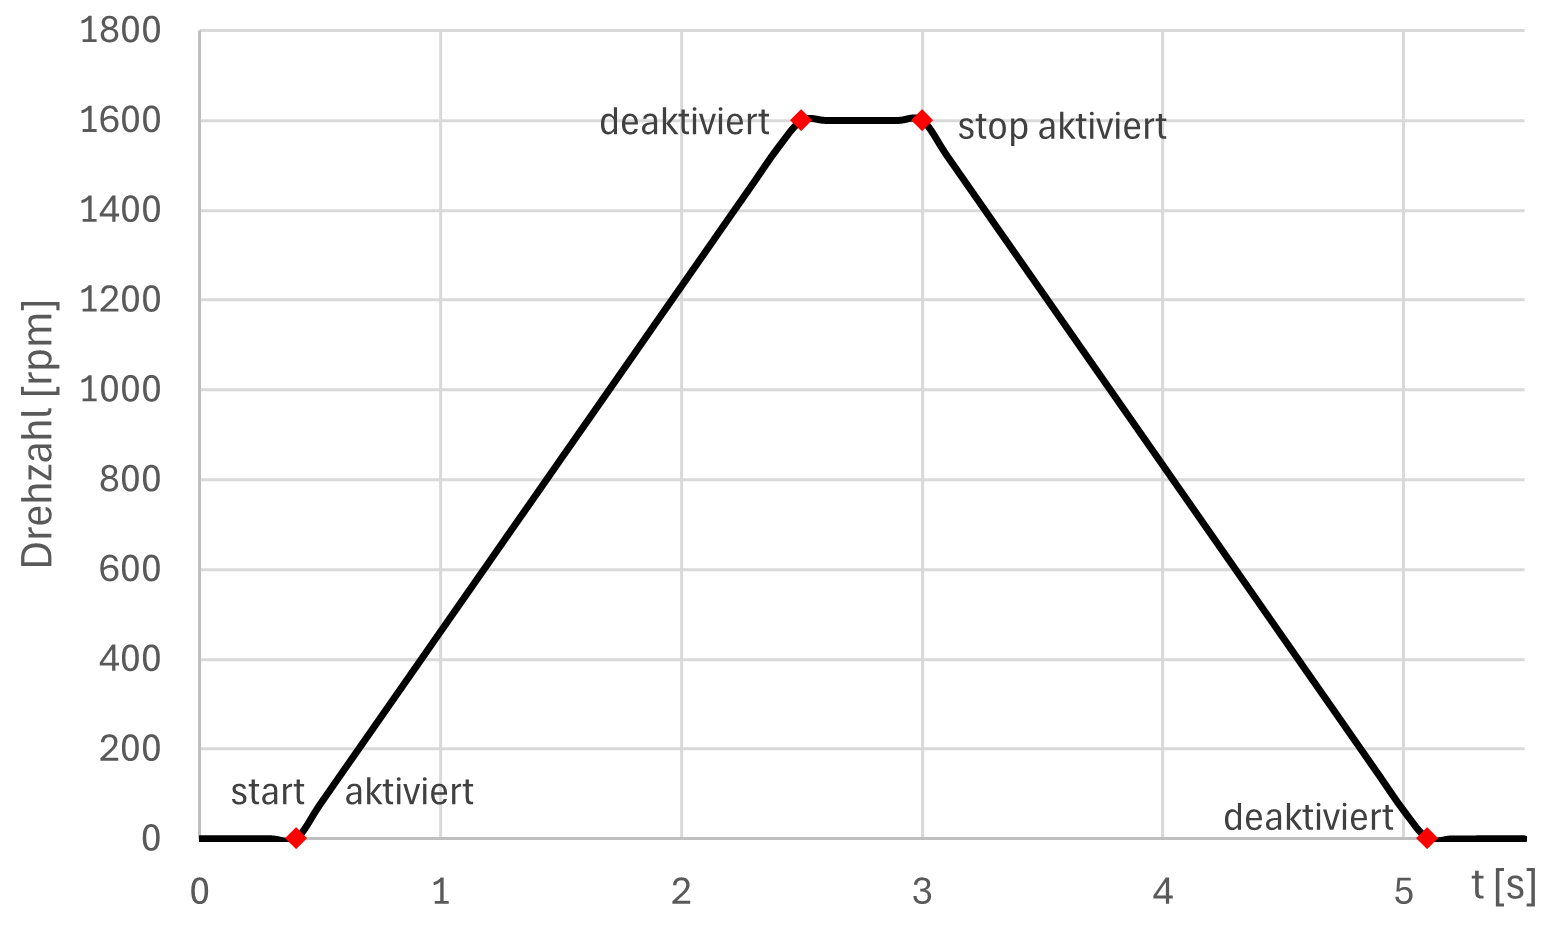
\includegraphics[width=0.75\linewidth]{images/Software/SpeedRamp.png}
	\caption{Drehzahlrampe: Beschleunigen und Bremsen}
	\label{fig:speedRamp}
\end{figure}
\noindent
Die Stopp-Funktion bietet zusätzlich die Möglichkeit über einen booleschen Parameter \verb|immediate| z.B. während einer Notabschaltung den Motor abrupt anzuhalten. In diesem Fall wird nicht die Rampe aktiviert sondern direkt die Motorfunktion \textit{Motor aus} gesetzt. 
\subsection{Steuerung der Linearführung}
nachdem die allgemeine Steuerung des Motors implementiert ist, gilt es, diese auf die Positionierung der Segel über die Linearführung anzuwenden. 
\subsubsection{Kalibrierung}\label{subsubsec:Kalibrierung}
Damit später eine bestimmte Stellung angefahren werden kann, muss die aktuelle Position jederzeit bekannt sein. Wie bereits erwähnt, dient das Puls-Signal des Motors als Maß, wie weit sich die Position von einem Startpunkt entfernt hat. Jedoch muss dieser Punkt erst angefahren werden, was durch die Detektion der Endschalter keine Schwierigkeit darstellt. Damit kann die absolute Position anhand der Puls-Zahl und der Gewindesteigung ermittelt werden. Für die Einstellung der Segel wird vom Controllino eine Prozentzahl vorgegeben wie weit gerollt oder getrimmt werden soll. Um diesen Wert auf eine absolute Position auf der Linearführung abzubilden, muss zusätzlich die Distanz zwischen den beiden Endpunkten ermittelt werden. Außerdem soll die Grenze zwischen Roll- und Trimmbereich nachträglich manuell angepasst werden können, um potenzielle Asymmetrien in der Seilführung der Segel auszugleichen. Der gesamte Ablauf der Kalibrierung wurde in Form einer Zustandsmaschine realisiert, wie in \autoref{fig:calibration} dargestellt.
\begin{figure}[H]
	\centering
	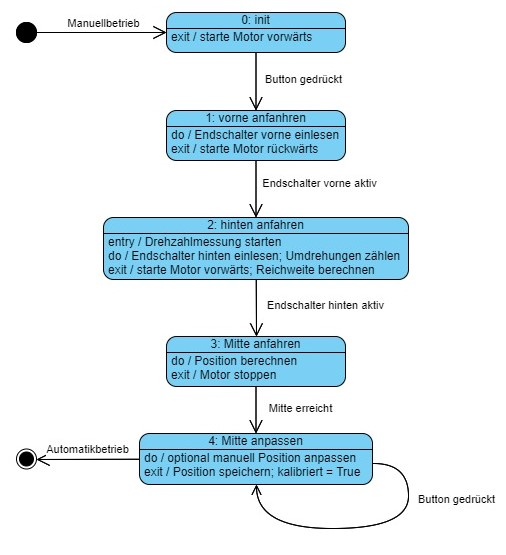
\includegraphics[width=0.8\linewidth]{images/Software/Kalibrierungsprozess.jpg}
	\caption{Kalibrierungsprozess}
	\label{fig:calibration}
\end{figure}
\noindent
Die Eintrittsbedingung der Kalibrierung ist das Einschalten des manuellen Betriebsmodus durch den Kippschalter am Gehäuse oder alternativ über den Webserver. Aus dem Ausgangszustand heraus muss der Knopf \textit{Speichern/Bestätigen} aus \autoref{fig:Bedienung} gedrückt werden, um die automatische Kalibrierung einzuleiten. Dies ist mit dem starten des Motors in Vorwärtsrichtung und dem Übergang in Zustand 1 verbunden. Anschließend wird der vordere Endschalter abgefragt, bis dieser aktiviert wird und die Endposition erreicht ist. Von dieser Position aus beginnt die Pulszählung, damit nach Ankunft am anderen Ende die zurückgelegte Distanz berechnet werden kann. Aus dieser Distanz wird daraufhin die Mitte bestimmt und angefahren. Ist diese erreicht, kann zuletzt die tatsächliche Grenze manuell über die Knöpfe \textit{Trimmen} und \textit{Rollen} angefahren und mit dem erneuten Druck des einleitenden Knopfes bestätigt werden. Als Feedback blinkt dabei die LED \textit{Position gespeichert}. Ebenso aktivieren bzw. deaktivieren sich nun nach der Einteilung der Bereiche je nach Positionierung die entsprechenden LEDs (\textit{Im Trimmungsbereich} / \textit{Im Rollbereich}).\\

\noindent
Da die Grenze in Zustand 4 mit dem entsprechenden Knopf beliebig oft angepasst werden kann, ist es durch das selbe Signal nicht möglich, den kompletten Prozess von vorne zu starten, ohne das System neu zu booten. Daher wurde ein Timer mit einem periodischen Callback konfiguriert, der die Dauer des Knopfdrucks ermittelt und ab einer Druckdauer von 3s die Zustandsmaschine zurücksetzt, anstatt lediglich die Grenze zu überschreiben. Nach Abschluss der Kalibrierung kann in den Automatikbetrieb gewechselt werden, indem der Controllino aufgrund der bereitgestellten Daten regelmäßig die optimale Segelstellung neu berechnet und an den stm32 zurückgibt. Der nächste Abschnitt beschäftigt sich damit, wie genau die gewünschte Segelstellung in eine Position auf der Linearführung umgerechnet wird. 
\subsubsection{Umsetzung einer Rollung/Trimmung}
Der Befehl einer Segelanpassung wird vom Controllino durch einen Modus (Rollen oder Trimmen) und eine Prozentzahl definiert. \autoref{fig:linearGuide} zeigt graphisch die Bedeutung dieser Angabe bezüglich der Positionierung an der Linearführung.
\begin{figure}[H]
	\centering
	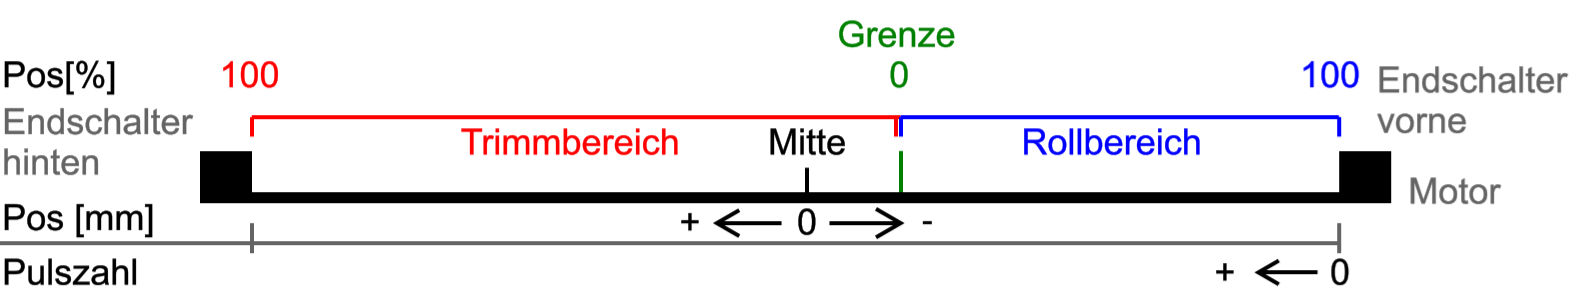
\includegraphics[width=\linewidth]{images/Software/LinearGuide.png}
	\caption{Rollung und Trimmung an der Linearführung}
	\label{fig:linearGuide}
\end{figure}
\noindent
In diesem Beispiel weicht die Grenze zwischen den beiden Bereichen stark von der tatsächlichen Mitte ab, um die Möglichkeit deren manuellen Anpassung, wie zuvor erwähnt zu verdeutlichen. Zur besseren Lesbarkeit der aktuellen Position wird diese in einem Zwischenschritt in mm umgerechnet und die Mitte der Gesamtdistanz auf null zentriert. In dieser Einheit werden jegliche Positionsberechnungen durchgeführt. \\

\noindent
Für die Umwandlungen zwischen Prozent, mm und Pulsen werden alle relevanten Daten in einer gleichnamigen Struktur des \verb|Localization|-Moduls festgehalten. \autoref{lst:sailAdjustment} zeigt die Ermittlung der gewünschten Position in mm mithilfe dieser Struktur aufgrund eines Segelanpassungsbefehls:
\begin{lstlisting}[language=C, caption={Berechnung der Zielposition}, label={lst:sailAdjustment}]
void Linear_Guide_set_desired_roll_trim_percentage(
	Localization_t *loc, uint8_t percentage, 
	adjustment_mode_t mode
)
{
	int8_t sign = mode == adjustment_mode_roll ? 1 : -1;
	int32_t roll_trim_distance = loc->end_pos_mm
	                           + sign * loc->center_pos_mm;
	loc->desired_pos_mm = (int32_t) 
	(- sign * (roll_trim_distance * (percentage / 100.0F)
	           - sign * loc->center_pos_mm));
}
\end{lstlisting}
Zunächst wird ein Vorzeichen \verb|sign| festgelegt, da der Rollbereich im negativen und der Trimmbereich im positiven mm Bereich liegt. Je nachdem welche Modus gewünscht ist, berechnet sich dessen Streckenanteil an der Linearführung aus der Distanz \verb|end_pos_mm| von der Mitte bis zu einem Endpunkt und dem Abstand \verb|center_pos_mm * sign| von der Mitte bis zur gewählten Grenze \verb|center_pos_mm|. Von dieser Strecke wird der gewünschte Anteil \verb|percentage| durch das Vorzeichen auf die richtige Seite orientiert. Zuletzt muss das addieren des Abstandes \verb|center_pos_mm * sign| wieder rückgängig gemacht werden.\\

\noindent
Nachdem die gewünschte Position in mm vorliegt, muss diese angesteuert werden. Dazu muss diese mit der aktuellen Position der Linearführung verglichen werden, welche sich nach der Kalibrierung aus der Pulszahl des Motors ergibt. Die Pulszahl wird wie bereits erwähnt durch den externen Interrupt am zuständigen GPIO-Pin regelmäßig aktualisiert und in der Struktur \verb|Localization_t| aus \autoref{lst:sailAdjustment} festgehalten. Die Positionsumrechnung ist in einer Funktion des \verb|Localization|-Moduls implementiert, wie nachfolgend gezeigt:
\begin{lstlisting}[language=C, caption={Positionsberechnung aus dem Pulssignal des Motors}, label={lst:pulseToPos}]
void Localization_update_position(Localization_t *loc)
{
	uint16_t abs_pos = loc->pulse_count
	                 * loc->distance_per_pulse;
	loc->current_pos_mm = abs_pos - loc->end_pos_mm;
}
\end{lstlisting}
Dabei berechnet sich die zurückgelegte Strecke pro Puls \verb|distance_per_pulse| aus dem Quotienten der Gewindesteigung von 1.12 mm pro Umdrehung und der Pulsfrequenz des Motors von 12 Pulsen pro Umdrehung zu 0.093 mm pro Puls.
\subsubsection{Optimierung der Bewegungsübergänge}
Die Steuerung der Linearführung wird durch das Aktivieren von Drehzahlrampen gelöst, um sanfte Beschleunigungs- und Bremsvorgänge zu ermöglichen. Allerdings gibt es unter dem bisherigen Stand der Implementierung mehrere Situationen, in denen es trotzdem noch zu abrupten Bewegungsänderungen kommt. Eine davon stellt das Erreichen eines Endpunktes dar, denn die Aktivierung des Endschalters ist direkt mit einem hardware-geregelten Stopp des Motors verbunden. Ebenfalls kann die Rampenfunktion nicht zwischen Beschleunigung in Vorwärts- und Rückwärtsrichtung unterscheiden, weshalb bei ein Befehl in die umgekehrte Richtung sofort umgesetzt wird. Ein anderes vielleicht noch wichtigeres Problem ist, dass eine gewünschte Position nicht korrekt angefahren werden kann, da der Motor nach dem Stopp-Befehl aufgrund der Rampe noch ein kleines Stück weiterfährt.\\

\noindent
Die Lösung dieser Probleme liegt in der Ermittlung des Bremsweges sowie der Einführung einer Warteschlange für Zielpositionen. Darauf basierend wurde ein Algorithmus zur optimierten Koordination der Steuerbefehle implementiert, wie nachfolgend in Form eines Programmablaufplans dargestellt:
\begin{figure}[H]
	\centering
	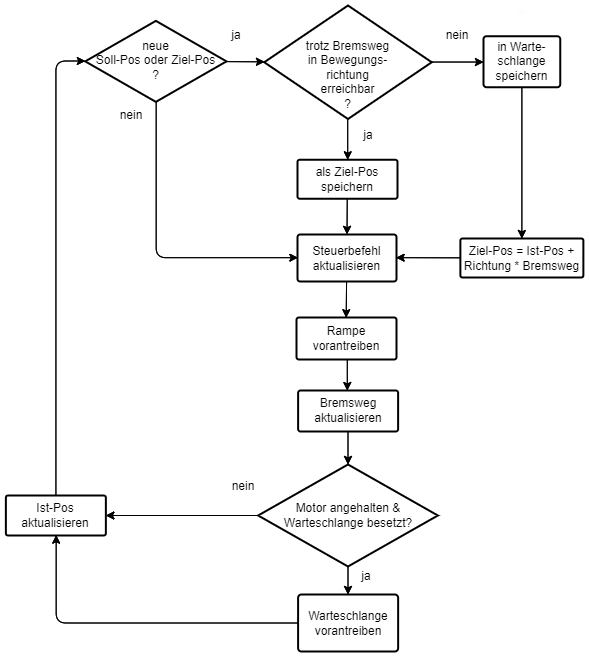
\includegraphics[width=\linewidth]{images/Software/ControlOptimization.png}
	\caption{Optimierung der Steuerbefehle}
	\label{fig:controlOptimization}
\end{figure}
\noindent
Eine Soll-Position kann entweder durch die manuelle Steuerung oder durch eine gewünschte Segelstellung vom Controllino während des Automatikbetriebs vorgegeben werden. Hat sich diese geändert, kann es sein, dass sich die Linearführung wegen eines vorhergegangenen Befehls bereits in Bewegung befindet. In diesem Fall muss überprüft werden, ob sich die Soll-Position in Bewegungsrichtung vor der aktuellen Position befindet und ggfs. ob der Abstand aufgrund des Bremsweges noch erreichbar ist. Wenn diese Bedingungen nicht erfüllt sind, wird die Soll-Position nicht direkt als neues Ziel gesetzt sondern in einer Warteschlange gespeichert, wobei diese eigentlich nur eine einzelne Variable der \verb|Localization_t| Struktur ist. Damit die neue Soll-Position trotzdem so schnell wie möglich erreicht wird, bildet der in Fahrtrichtung nächste noch erreichbare Punkt die neue Zielposition. Danach kann der Steuerbefehl aktualisiert werden (Vorwärts, Rückwärts oder anhalten). Nach Vorantreiben der Rampe muss der Bremsweg aufgrund der aktuellen Drehzahl ebenfalls neu berechnet werden. Ist der Motor zum Stillstand gekommen, kann sofern vorliegend die Position aus der Warteschlange als neues Ziel vorgerückt werden. Zuletzt muss natürlich auch die aktuelle Position der Linearführung aktualisiert werden bevor der Kreislauf von neuem beginnt. \\

\noindent
Sollte eine Soll-Position auch nach einem Richtungswechsel aufgrund einer Fehlberechnung des Bremsweges verfehlt werden, wird diese einfach erneut in die Warteschlange gesetzt, sodass sich die exakte Position garantiert einpendelt. Zusammenfassend werden nun mithilfe der Ziel-Warteschlange abrupte Richtungswechsel vermieden und durch die Berechnung des Bremsweges kann das System rechtzeitig anhalten, um die Soll-Position präzise anzufahren oder den Aufprall am Endschalter zu verhindern.
\subsubsection{Wiederherstellung der Position}
Die in Kapitel \ref{subsubsec:Kalibrierung} beschriebene Kalibrierung ist ein zeitintensiver Prozess. Damit diese nicht bei jedem Programmneustart erneut durchgeführt werden muss, wurde ein FRAM Speicher in der Hardware verbaut, um dort alle relevanten Informationen zur Wiederherstellung der aktuellen Position hineinzuschreiben und bei Bedarf wieder auszulesen. Für diese beiden Funktionen wurde ein Benutzerinterface im \verb|FRAM|-Modul implementiert.\\

\noindent
Das \ac{FRAM} Modul steuert den \ac{FRAM} über \ac{SPI} an. Der FRAM kann dabei über sechs Befehle gesteuert werden. Dabei wurden die Befehle: WREN(0000 0110b), RDSR(0000 0101b), READ(0000 0011b) und WRITE(0000 0010b) genutzt. Um auf den Speicher zu schreiben wird das \ac{WREN} Bit gesetzt. Hierfür wird der gleichnamige Befehl genutzt. Um zu überprüfen ob das Bit gesetzt wurde, wird mit dem Befehl RDSR das Status Register ausgelesen und das Bit 7 überprüft. Um auf den Speicher zu schreiben wird mit dem WRITE Befehl gefolgt von einer 12Bit Addresse der Speicherbereich ausgewählt. Die Darauffolgenden Bits werden in den Speicher geschrieben. Beim auslesen mit dem Befehl READ ist das vorgehen gleich, nur werden hier keine zusätzlichen Bits übertragen. In der Software wurden dabei die zwei Funktionen \verb|FRAM_write| und \verb|FRAM_read| erstellt die für einen high level access sorgen. Über diese kann ein Puffer in den \ac{FRAM} geschrieben werden oder die Daten ausgelesen werden. Die Serialisierung und Deserialisierung, sowie das setzen des \ac{WREN} Bits wird beim Aufruf übernommen.\\

\noindent
Damit die Daten beim Auslesen zur Initialisierung des Systems aktuell sind, werden diese bei jeder Positionsänderung an der entsprechenden Speicheraddresse überschrieben. Die für die Lokalisierung nötigen Informationen werden zur Serialisierung innerhalb einer separaten Struktur organisiert, wie nachfolgend gezeigt:
\begin{lstlisting}[language=C, caption={Speicherformat der Positionsdaten}, label={lst:locSafeData}]
typedef struct {
	Loc_state_t state;
	int16_t pulse_count;
	uint16_t end_pos_mm;
	int16_t center_pos_mm;
	uint16_t start_pos_abs_mm;
} Loc_safe_data_t;
\end{lstlisting}
Die bisher nicht eingeführte Variable \verb|start_pos_abs_mm| entspricht dem vom Distanzsensor gemessenen Abstand der Position bei Aktivierung des vorderen, motor-seitigen Endschalters. Daraus lässt sich die mit dem Puls-Signal ermittelte Position mit dem Messwert des Sensors vergleichen. Die Bedeutung der Messung wird in Kapitel \ref{subsubsec:Fehlerbehandlung} genauer behandelt. \\

\noindent
Der Schreibprozess dieser Daten in das FRAM ist durch eine Funktion \\\verb|Linear_Guide_safe_Localization()| gegeben. \autoref{lst:safeLocalization} zeigt deren Implementierung.
\begin{lstlisting}[language=C, caption={FRAM Speichervorgang}, label={lst:safeLocalization}]
int8_t Linear_Guide_safe_Localization(Localization_t loc)
{
	uint8_t FRAM_buffer[sizeof(Loc_safe_data_t)];
	Localization_serialize(loc, FRAM_buffer);
	if(FRAM_write(FRAM_buffer, 
	              LINEAR_GUIDE_INFOS, 
	              sizeof(Loc_safe_data_t)) != HAL_OK)
	{
		printf("Saving Position failed!\r\n");
		return LG_LOCALIZATION_FAILED;
	}
	return LG_LOCALIZATION_SAFED;
}
\end{lstlisting}
Zunächst wird ein FRAM-Puffer der Größe des Speicherformats aus \autoref{lst:locSafeData} deklariert. Dann werden die entsprechenden Daten in der Funktion\\ \verb|Localization_serialize()| von der Struktur \verb|loc| in das richtige Format extrahiert und anschließend an den Puffer adressiert. Zuletzt werden die Daten innerhalb des Puffers durch \verb|FRAM_write()| an die definierte Addresse\\ \verb|LINEAR_GUIDE_INFOS| des physischen Speichers transferiert.\\

\noindent
Nachdem die Daten während des Betriebs kontinuierlich im FRAM aktualisiert werden, können diese bei einem Neustart des Systems in umgekehrter Weise wie in \autoref{lst:safeLocalization} durch \verb|FRAM_read()| abgerufen werden. \autoref{lst:deserialize} zeigt die Verarbeitung des resultierenden Ausgangspuffers \verb|buffer|:
\begin{lstlisting}[language=C, caption={Auslesen der Positionsdaten aus dem FRAM-Puffer}, label={lst:deserialize}]
static int8_t Localization_deserialize(
	Localization_t *loc, 
	uint8_t buffer[sizeof(Loc_safe_data_t)]
)
{
	Loc_safe_data_t *data = (Loc_safe_data_t *)
		malloc(sizeof(Loc_safe_data_t));
	memcpy(data, buffer, sizeof(Loc_safe_data_t));
	loc->state = data->state;
	loc->pulse_count = data->pulse_count;
	loc->end_pos_mm = data->end_pos_mm;
	loc->center_pos_mm = data->center_pos_mm;
	loc->start_pos_abs_mm = data->start_pos_abs_mm;
	free(safe_data_ptr);
	if (loc->state != Loc_state_5_center_pos_set)
	{
		return LOC_RECOVERY_RESET;
	}
	return LOC_RECOVERY_COMPLETE;
}
\end{lstlisting}
Im ersten Schritt wird ein Pointer \verb|data| im Speicherformat \verb|Loc_safe_data_t| entsprechend allokiert, damit diesem anschließend mit der c-Standard-Funktion \verb|memcpy()| die Daten aus dem Puffer übertragen werden können. Danach werden die einzelnen Werte der Reihe nach der Hauptstruktur des \verb|Localization|-Moduls übergeben. Zuletzt wird mit der \verb|state|-Variable überprüft, ob die Kalibrierung beim letzten Betrieb abgeschlossen wurde. Falls nicht, muss diese wiederholt werden, was das Rückgabe-Flag \verb|LOC_RECOVERY_RESET| signalisiert. War die Wiederherstellung der Lokalisierung erfolgreich, kann die aktuelle Position wie gehabt entsprechend \autoref{lst:pulseToPos} mit den Werten \verb|pulse_count| und \verb|end_pos_mm| ermittelt werden. Durch das Speichern der Grenze \verb|center_pos_mm| bleiben außerdem auch die zuvor eingestellten Trimm- und Rollbereiche erhalten.
\subsubsection{Fehlerbehandlung}\label{subsubsec:Fehlerbehandlung}
Mithilfe der Sensoren und dem Fehlersignal des Motors können verschiedene Fehlerzustände identifiziert werden. \autoref{tab:Fehlerbehandlung} listet diese auf, stellt deren Bedingung dar und wie damit umgegangen wird.
\begin{table}[H]
	\centering
	\begin{tabular}{|c|c|c|c|}
		                                                                                    \hline
		\textbf{ID} & \textbf{Bezeichnung} & \textbf{Bedingung}  & \textbf{Behandlung}   \\ \hline
		0           & Normal               & kein Fehler         & keine                 \\
		            &                      & identifiziert       &                       \\ \hline
		1           & Distanzfehler        & Toleranz von 1 cm   & Anpassung an Messwert \\
		            &                      & zwischen Messwert   &                       \\
		            &                      & und Pulsberechnung  &                       \\
		            &                      & überschritten       &                       \\ \hline
		2           & Windfehler           & max. Geschwindigkeit& Segel 100 \% einrollen\\
		            &                      & überschritten       &                       \\ \hline
		3           & Motorfehler          & Fehlersignal aktiv  & Notabschaltung        \\ \hline
		4           & Stromfehler          & Stromsensorwert von & Notabschaltung        \\
		            &                      & 4 A überschritten   &                       \\ \hline
	\end{tabular}%
	\caption{Fehlerzustände}
	\label{tab:Fehlerbehandlung}
\end{table}
\noindent
Bei jedem Fehler leuchtet als Feedback die LED \textit{Störung} aus \autoref{fig:Bedienung} auf. Während Fehler 1 vom System automatisch korrigiert werden kann, wird bei den anderen im Gegensatz dazu der weitere Betrieb solange blockiert, bis diese behoben sind. Die Toleranz zur maximalen Windgeschwindigkeit soll dabei vom Controllino festgelegt werden, da dort auch die Berechnungen zur optimalen Segelstellung durchgeführt werden. Daher wird der Windfehler auch nicht vom STM32 selbst gesetzt, sondern vom Controllino über das REST-Protokoll kommuniziert.
\subsection{Windmessung mit dem Anemometer}
Wie bereits in \autoref{Mangelnde_Präzision} aufgezeigt war die Präzision der Analogen Signale zwar ausreichend aber teilweise sehr ungenau. Aus diesem Grund wurde stattdessen die digitale RS485 Schnittstelle zur Übertragung der Windgeschwindigkeit und Windrichtung genutzt. Der WSWD bietet dabei mehrere Protokolle an, um diese Daten Formattiert zu übertragen. Dabei wurde das \ac{NMEA} Telegramm ausgewählt. Die Formatierung ist in \autoref{fig:NMEA_Protokoll} dargestellt.
\begin{figure}[H]
	\centering
	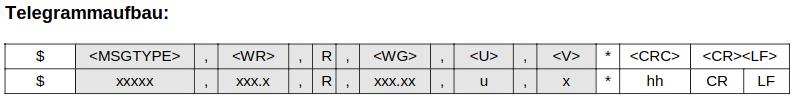
\includegraphics[width=\linewidth]{images/Software/NMEA_Telegramm_Aufbau.png}
	\caption{Aufbau eines NMEA Telegramm aus \cite{WSWD}, S.61}
	\label{fig:NMEA_Protokoll}
\end{figure}
\noindent Hier wird neben den Daten ($<WR>$ und $<WG>$) ebenfalls die Gültigkeit der Messung ($<V>$) und die Einheit der Geschwindigkeit ($<U>$) übertragen. Das versenden von Befehlen geschieht dabei aber in einem von MESA selbsterstellten Format:
\begin{table}[H]
	\centering
	\begin{tabular}{|l|l|l|l|}
		\hline
		\textbf{\textless{}ID\textgreater{}} & \textbf{\textless{}CM\textgreater{}} & \textbf{\textless{}PARAM\textgreater{}} & \textbf{\textless{}CR\textgreater{}\textless{}LF\textgreater{}} \\ \hline
		Geräte ID                            & Kommando                             & Parameter                               & Befehlsabschluss                                                \\ \hline
	\end{tabular}
	\caption{}
	\label{tab:my-table}
\end{table}
\noindent Dieses wird im Normal Betrieb nicht benötigt, aber kann zur einmaligen Konfiguration des Sensors genutzt werden. Zur Konfiguration des Anemometers wurde z.b dabei der Befehl 42 angwewandt um die bereits Erklärten \ac{NMEA} Telegramme in einem regelmäßigen Abstand gesendet zu bekommen.

\noindent Die Befehle an das Anemometer werden über \ac{UART} Gesendet und Empfangen. Das Signal wird dann vom MAX3485 zu RS485 konvertiert. Da RS485 nur eine Halbduplex Kommunikation zulässt muss vorher über das Setzen eines Pins immer zwischen Senden und Empfangen gewechselt werden. Dies wurde in zwei Funktionen: \verb|WSWD_enable_receive| und \verb|WSWD_enable_send| realisiert. Diese prüfen zuerst den Status des Pins und ändern diesen falls nötig. Diese werden in den Sende und Empfangs Funktionen genutzt. Diese Serialisieren/Deserialisieren eine Zeichenkette mit einem Cast zu \verb|uint8_t*| und Versenden/Empfangen diese über die \verb|HAL_UART_Transmit|/\verb|HAL_UART_Receive| Funktionen:
\begin{lstlisting}[language=C, caption={Empfangen einer Nachricht vom WSWD}, label={lst:WSWDreceive}]
uint8_t WSWD_receive
(char* receive_buffer, uint8_t size_of_receive_buffer)
{
	WSWD_enable_receive();
	if(HAL_UART_Receive(&huart2, (uint8_t*)receive_buffer, 
	size_of_receive_buffer, WSWD_UART_TIMEOUT) != HAL_OK)
	{
		printf("error sending to WSWD\r\n");
	}
	return HAL_OK;
}
\end{lstlisting}
Beim Empfangen der Daten wird das komplette Telegramm als ein String gespeichert. Die Telegramm Struktur wird danach durch String Manipulation geprüft und die gesendeten Daten über die \verb|atof| Funktion zu einem nutzbaren \verb|float| Datentyp Konvertiert. Dasselbe Prinzip wird auch beim Versenden eines Befehles angewandt, nur das hier der String mit \verb|snprintf| zusammengesetzt wird.\\
\subsection{\ac{REST} Interface}
Das \ac{REST} Interface wird genutzt um mit dem Controllion zu kommunizieren. Zuerst wurden die hierfür benötigten \ac{HTTP} Befehle festgelegt. Da der Controllino als Client agieren soll und somit immer der Initiator der Kommunikation ist wurden die Befehle: \verb|GET| und \verb|PUT| als ausreichend angesehen. Die dabei mit versendeten Daten sollen im \ac{JSON} Format versendet werden. Die \verb|URL| auf die der Controllino über die \ac{API} zugreift wurden ebenfalls festgelegt. Diese wurden nach den unterschiedlichen Daten organisiert. Um z.B alle Daten abzufragen sendet der Controllino den Befehl: \verb|GET /data|. Sollte er speziellere Infos abfragen wollen, wie z.B die Segelposition, sendet er den Befehl: \verb|GET /data/adjustment|. Eine Übersicht aller validen \ac{URL}s und JSON Formatierungen ist in \autoref{sec:REST} zu finden. Ein Beispiel für ein Antwort Paket für den \verb|GET /data/adjustment| ist in \autoref{lst:JSONantwort} zu sehen.
\begin{lstlisting}[language=C, caption={GET /data/adjustment Antwort Paket}, label={lst:JSONantwort}]
{
	"sail_pos": <(int) pitch/roll [+/- 0...100 %]>
}
\end{lstlisting}
Über den \verb|PUT| Befehl kann der Controllino einen Fehler setzen, eine gewünschte Position anfahren oder den Betriebsmodus der Steurung ändern. Zusätzlich kann auch der maximale Distanz Fehler und die maximale Drehzahl des Motors festgelegt werden.\\

\noindent Zur Netzwerkkommunikation wurde der \ac{LWIP} Stack genutzt. Dieser beinhaltet allerdings keine bereits integrierte \ac{REST} \ac{API}. Aus diesem Grund wurde diese selbst implementiert. Dabei wurde ein \ac{TCP} Server erstellt. Dieser wird auf dem Mikrocntroller gehostet. Dieser nimmt die Rohdaten aus den Empfangen Paketen und speichert diese in einem Buffer. Der Buffer wird daraufhin an die \ac{REST} \ac{API} weitergegeben. Diese unterscheidet dabei zwischen den zwei möglich Befehlen und den akzeptierten \ac{URL}s. Falls diese nicht stimmen wird mit dem \ac{HTTP} Error code \verb|404 Not Found| geantwortet. Falls es sich um einen \verb|PUT| Befehl handelt, wird der mitgesendete JSON Payload auf eine Korrekte Formattierung geprüft. Hierfür wurde die cJson Bibliothek genutzt. Je nachdem ob die Formattierung stimmt wird mit \verb|200 OK| oder mit \verb|501 Not Implemented| bzw. \verb|400 Bad Request| geantwortet.\\

\noindent Beim versenden einer Antwort auf eine \verb|GET| Request wird ebenfalls mit Hilfe der cJson Bibliothek ein Payload zusammengebaut, der die aktuellen angeforderten Werte beinhaltet. Der festgelegte Port 
\subsection{Weboberfläche}
Der Webserver stellt eine alternative zu der physikalischen Bedienungsoberfläche dar. Damit für Einstellungen, Wartung und Überwachung nicht jedes mal auf die Kuppel gestiegen werden muss, wurde ein Weboberfläche hinzugefügt.
\subsubsection{Funktionalität}
Die Weboberfläche, soll es einer Arbeitskraft erlauben den aktuellen Status, sowie Einstellungen des Gerätes abzufragen oder festzulegen. Dabei sollen dieselben Informationen, die der Controllino über die \ac{REST} \ac{API} abfragen kann auch auf diesem dargestellt werden. Zusätzlich dazu soll es hier auch möglich sein, dieselbe Funktionalität wie die Benutzeroberfläche zu bieten. Also sollte es möglich sein manuell über die Weboberfläche die Segel zu Rollen und zu Trimmen. Dazu gehört auch die Auslösung einer Kalibrierungsfahrt.
Die Netzwerkeinstellungen sollten ebenfalls über die Weboberfläche gesetzt werden können. Dazu zählen die Aktivierung von DHCP, das festlegen einer IP-Adresse und das zurücksetzen dieser.
\subsubsection{Webseiten}
Die Webseiten wurden dabei nach ihrem Inhalt sortiert. Es wurden insgesamt sechs Seiten implementiert:
\begin{itemize}
	\item Index Seite
	\item Positionsdaten Seite
	\item Sensordaten Seite
	\item Einstellungs Seite
	\item Error Seite
	\item Login Seite
\end{itemize}
Als Beispiel ist die Index Seite in \autoref{fig:HTMLindex} dargestellt.
\begin{figure}[H]
	\centering
	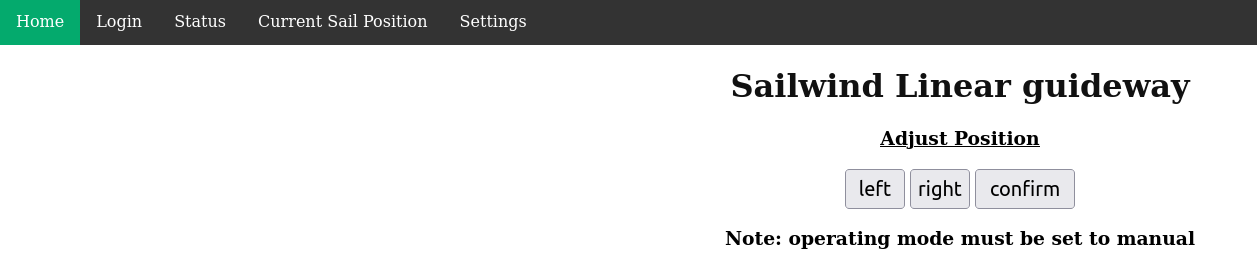
\includegraphics[width=\linewidth]{images/Software/Html_index_seite.png}
	\caption{Index Seite des Webservers}
	\label{fig:HTMLindex}
\end{figure}
\noindent Hier befindet sich die manuelle Steuerung zur Positionierung der Segel. Auf allen Seiten wird dabei am oberen Rand eine Navigations Bar angezeigt mit der zu den anderen Seiten Navigiert wird. Auf der Positionsdaten Seite ist der aktuelle Betriebsmodus und die Trimmung/Rollung der Segel zu finden. Die Sensordaten Seite zeigt alle aktuellen Werte der Sensoren an und wird regelmäßig aktualisiert. Die Einstellungsseite zeigt die aktuellen Einstellungen und macht es möglich den Betriebsmodus zu ändern, das Gerät neuzustarten und eine neue IP Adresse festzulegen oder \ac{DHCP} zu aktivieren. Die Login Seite hat aktuell keine Funktion und dient nur als Platzhalter. Hier könnten später je nach Nutzer die aufrufbaren Webseiten eingeschränkt werden. So kann z.B ein Service Mitarbeiter auf alle Einstellungen zugreifen, während ein normaler Nutzer nur z.B die Sensordaten abfragen kann. Die Error Seite wird nur bei einer Zeitüberschreitung der Anfrage angzeigt und hat keinen weiteren Nutzen.
\subsubsection{Umsetzung}
Die Webserver erhält dieselbe \ac{IP} Adresse wie die \ac{REST} \ac{API} ist aber auf dem Port 80 erreichbar. Im Gegensatz zum \ac{REST} interface bietet \ac{LWIP} hier bereits schon eine fertige Webserver implementierung. Dabei können Daten über die \ac{SSI} und \ac{CGI} Handler Übertragen werden. Beim Aufrufen einer Webseite werden die im \ac{HTML} Code festgelegten \ac{SSI} Tags mit den entsprechenden Sensor Daten oder Text mit einer Rückmeldung für den User ersetzt. Hierfür wurde ein zentrales \verb|switch-case| festgelegt, das nach der Nummer des \ac{SSI} Tags unterscheidet und den dementsprechend String einfügt. Der \ac{CGI} Handler wird für Textboxen oder für Buttons genutzt. Für Buttons wurden dafür \ac{HTML} Forms genutzt. Diese haben als \verb|Action| einen \ac{URI} wie in \autoref{lst:URI} zusehen ist. 
\begin{lstlisting}[language=C, caption={GET /data/adjustment Antwort Paket}, label={lst:URI}]
	<form action="/form_control.cgi">
	<p>
	<input type="submit" 
	id="move" 
	value="confirm" 
	name="move" 
	style="width:100px;height:40px;font-size:20px;">
	</p>
	</form>
\end{lstlisting}
Wird jetzt z.B auf der Index Seite der Button \glqq{}Confirm\grqq{} angeklickt wird der String: \verb|/form_control.cgi?move=confirm| zum Mikrocontroller gesendet. Auf Basis dieses String kann daraufhin eine Aktion gewählt werden und z.B die Anzeige auf dem Webserver verändert werden. Textinputs funktionieren ähnlich nur das sie den Inhalt der Textbox nach der \ac{URI} beinhalten.





        \section{Fazit und Ausblick}
Abschließend kann für diese Arbeit festgehalten werden, dass die neue Schnittstelle erfolgreich implementiert und getestet wurde. Der Tankautomat ist jetzt in der Lage über das OCPP Protokoll Verbindungen zu Ladesäulen herzustellen und Ladevorgänge zu verwalten. Dabei konnte während der Konzeption durch die Analyse der Abläufe die benötigten Nachrichten und Konfigurationsparameter ermittelt werden. Mit diesem Vorgehen wurde für eine kürzere Umsetzungszeit und weniger Aufwand gesorgt. Aufgrund des kleinen benötigten Umfanges und der unbefriedigenden Auswahl an fertigen Lösungen, wurde sich für eine Selbstentwicklung des Protokolls entschieden, die auf der Basis der Websocketpp Bibliothek aufgebaut wurde. Durch die komplette eigene Entwicklung der Erweiterung konnte ebenfalls dafür gesorgt werden, dass zukünftig auch eine Verschlüsselung der Kommunikation und die Erweiterung des Protokollumfang einfach zu gestalten sind. Die Ergänzung der Weboberflächen Felder wurde genutzt um einfach die Ladesäulen identifizieren zu können und hilft dem Kunden die Ladesäulen individueller zu konfigurieren. Mit dieser Basis konnte der Umsetzungsplan entworfen werden. Dieser konnte dann während der Implementierung angewandt und umgesetzt werden. Dabei gab es allerdings unvorhergesehene Probleme mit den Protokollabläufen der OCPP2.0.1 Version, die aber Dank der Tests auffielen und schnell behoben werden konnten. Abschließend wurde mithilfe der Tests, am Großteil der Ladesäulen, verifiziert, dass die Anforderungen erfüllt wurden. Es muss aber in Folge der Komplikationen mit der Wallbe Ladesäule noch weiter nach dem Grund der Inkompatibiliät gesucht werden. In Zuge dessen sollten die Tests in Zukunft weiter ausgebaut und automatisiert werden, damit auch weitere Sonder- und Randfälle abgedeckt sind. Dafür wurden Empfehlungen und mögliche Vorgehensweisen dargelegt die in der Zukunft vom Entwicklerteam umgesetzt werden. 
\newline




    \backmatter %-------------------------------------------------
    \nonumcontent{Literaturverzeichnis}
\printbibliography
    \appendix
\section{Schaltpläne}
\label{sec:Schaltplan}
\subsection{Schaltplan Übersicht}
\begin{figure}[H]
	\centering
	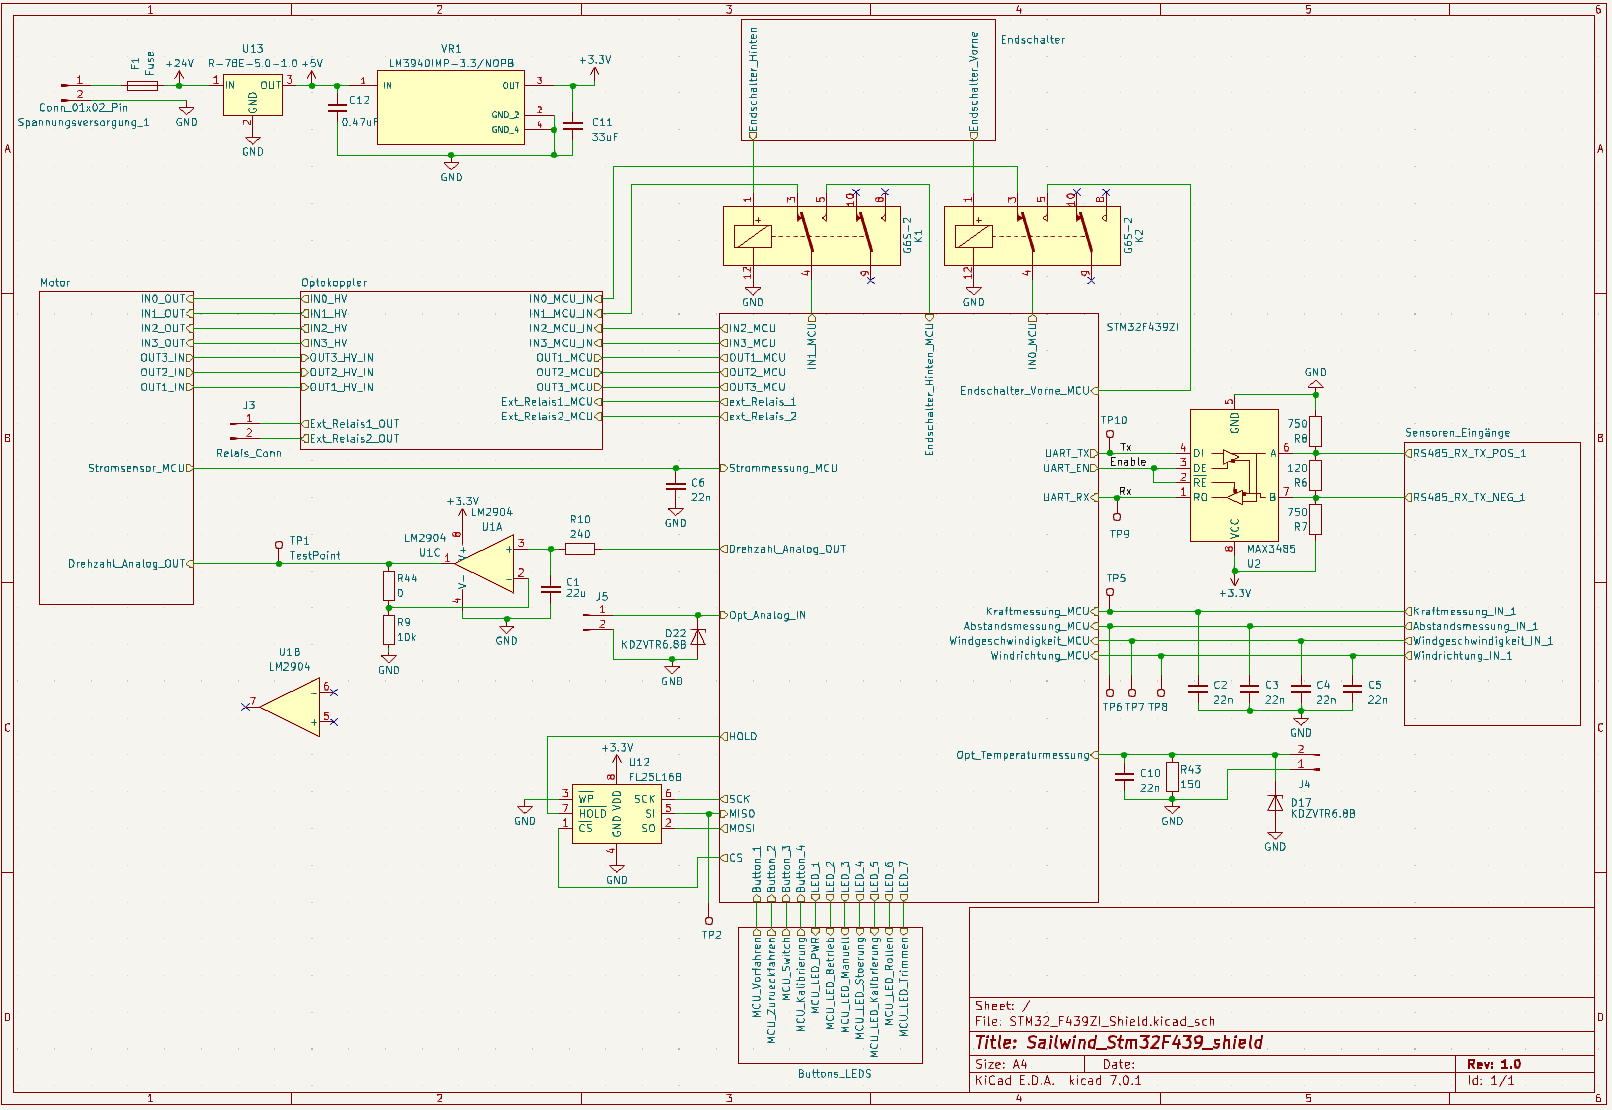
\includegraphics[width=1.0\textwidth]{images/Hardware/Schaltplan_Gesamt.PNG}
	\caption{Schaltplan Übersicht}
	\label{fig:Schaltplanuebersicht}\begin{center}
	\end{center}
\end{figure}
\subsection{Schaltplan STM32F439 Gruppe}
\begin{figure}[H]
	\centering
	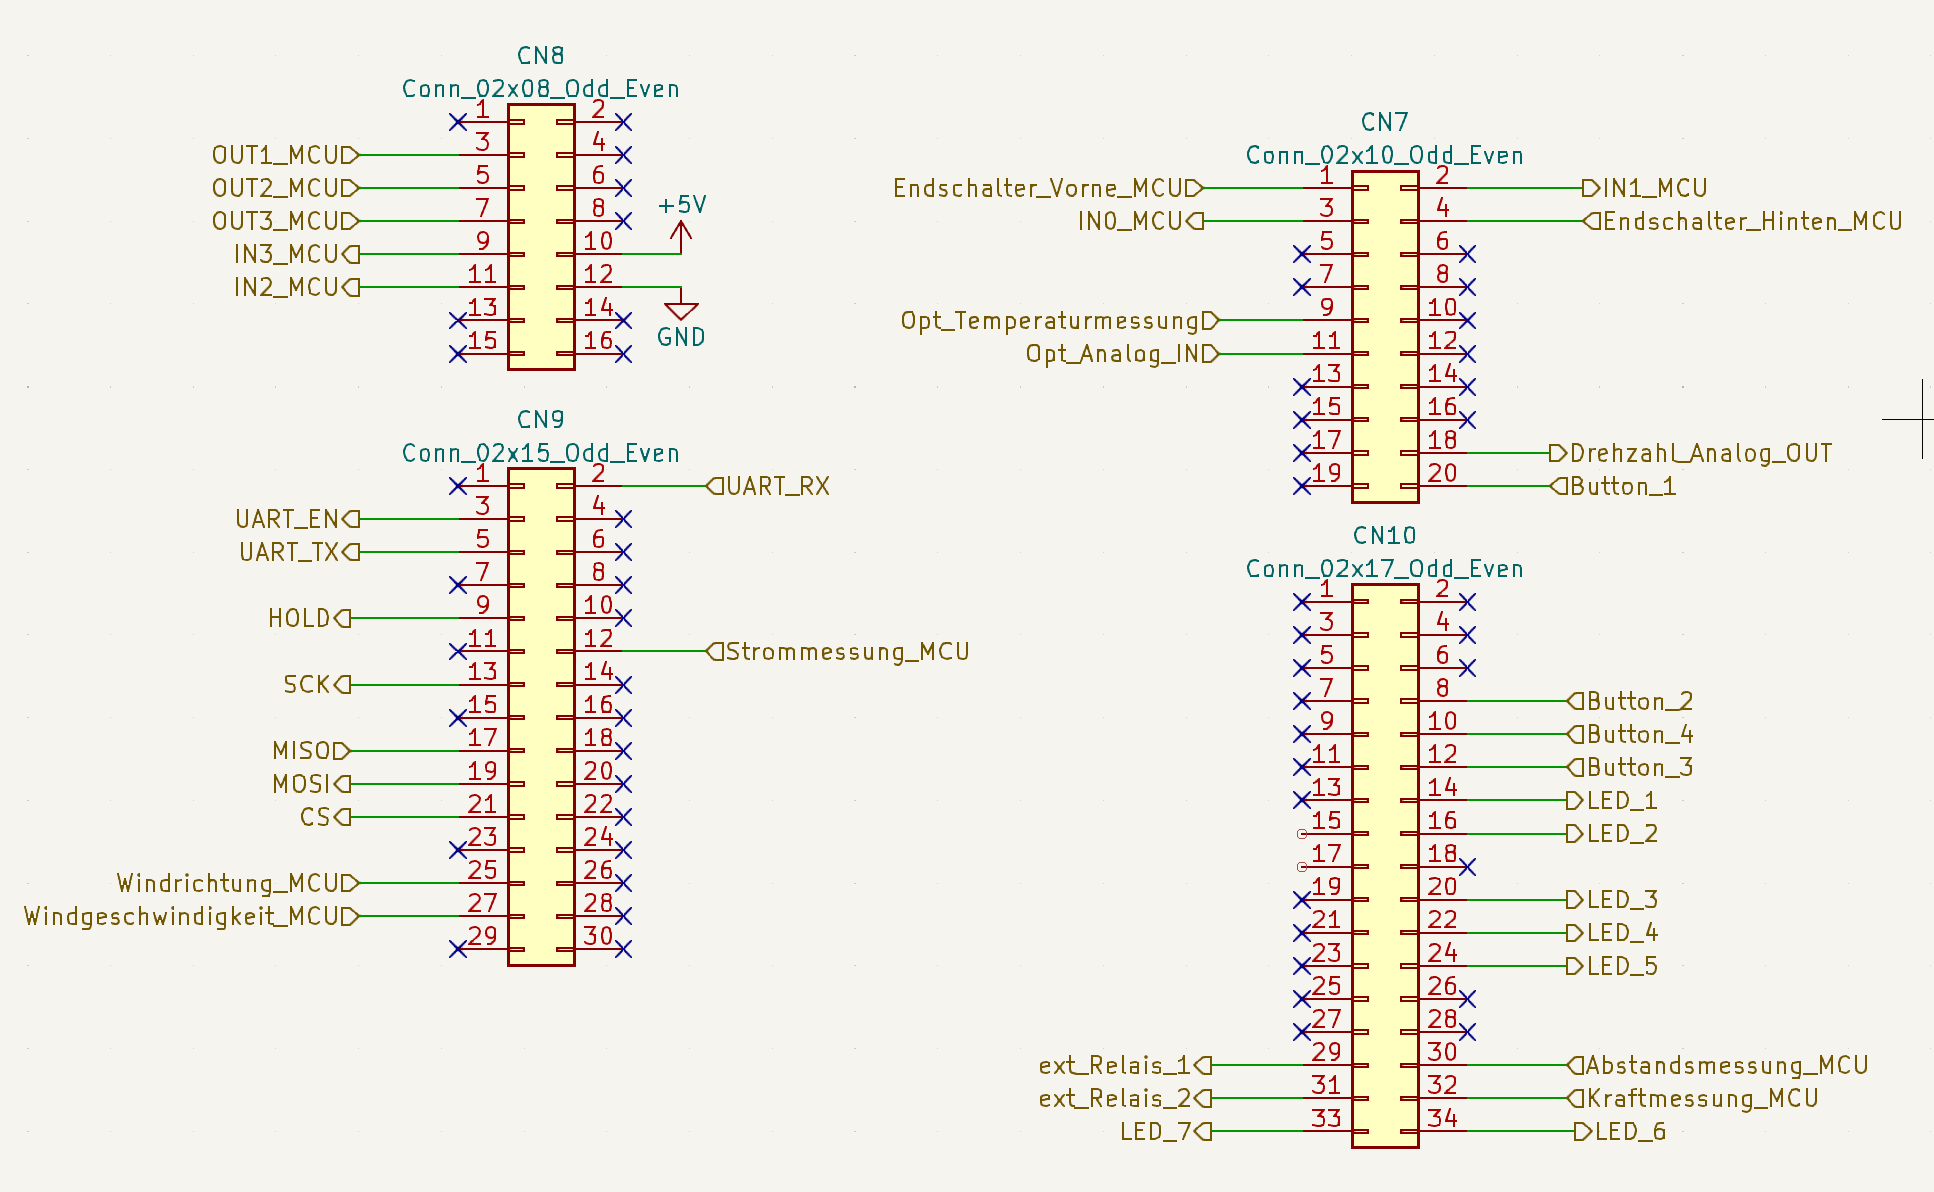
\includegraphics[width=1.0\textwidth]{images/Hardware/Schaltplan_STM32.PNG}
	\caption{Schaltplan der STM32F439 Gruppe}
	\label{fig:STM32Gruppe}\begin{center}´
	\end{center}
\end{figure}
\subsection{Schaltplan Buttons und LED Gruppe}
\begin{figure}[H]
	\centering
	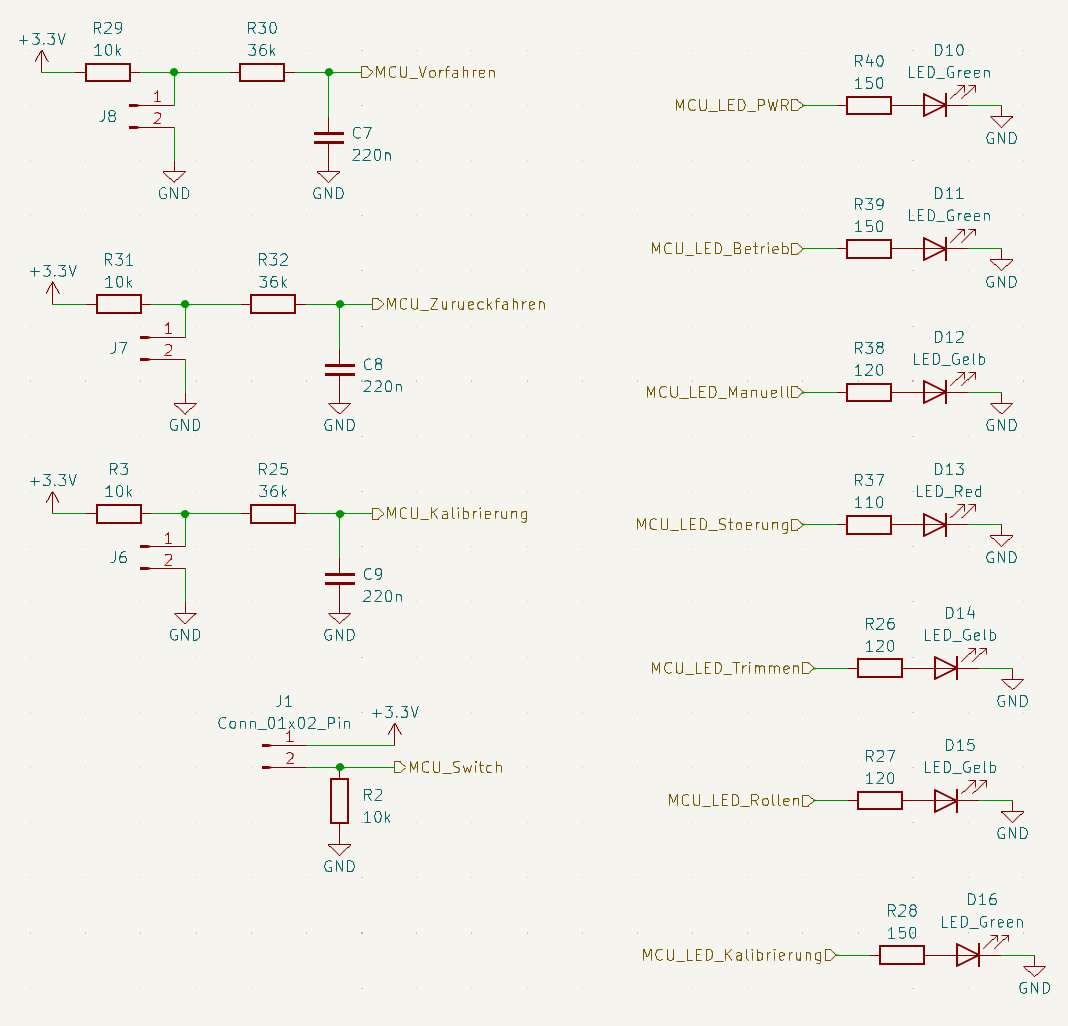
\includegraphics[width=1.0\textwidth]{images/Hardware/LEDS_und_buttons_schaltplan.PNG}
	\caption{Schaltplan der Buttons und LED Gruppe}
	\label{fig:ButtonGruppe}\begin{center}
	\end{center}
\end{figure}
\subsection{Schaltplan Sensoren Gruppe}
\begin{figure}[H]
	\centering
	\includegraphics[width=1.0\textwidth]{images/Hardware/Sensoren_Eingänge_Schaltplan.PNG}
	\caption{Schaltplan der Sensoren Gruppe}
	\label{fig:SensorenGruppe}\begin{center}
	\end{center}
\end{figure}
\subsection{Schaltplan Motor Gruppe}
\begin{figure}[H]
	\centering
	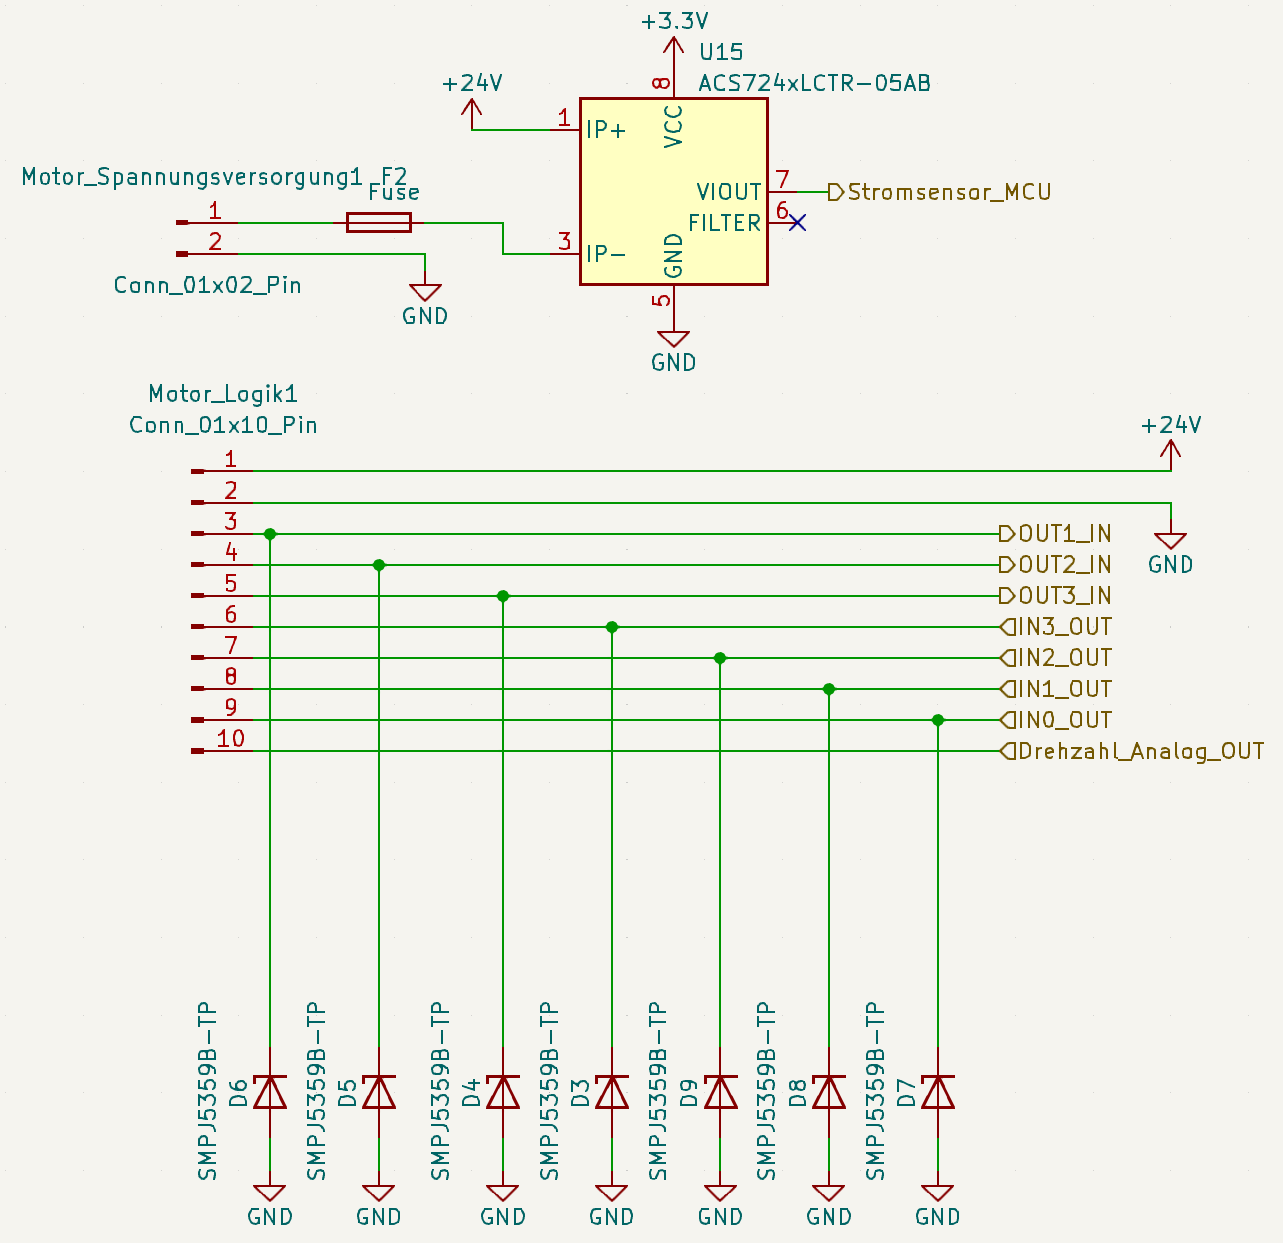
\includegraphics[width=1.0\textwidth]{images/Hardware/Motor_Schaltplan.PNG}
	\caption{Schaltplan der Motor Gruppe}
	\label{fig:MotorGruppe}\begin{center}
	\end{center}
\end{figure}
\subsection{Schaltplan Endschalter Gruppe}
\begin{figure}[H]
	\centering
	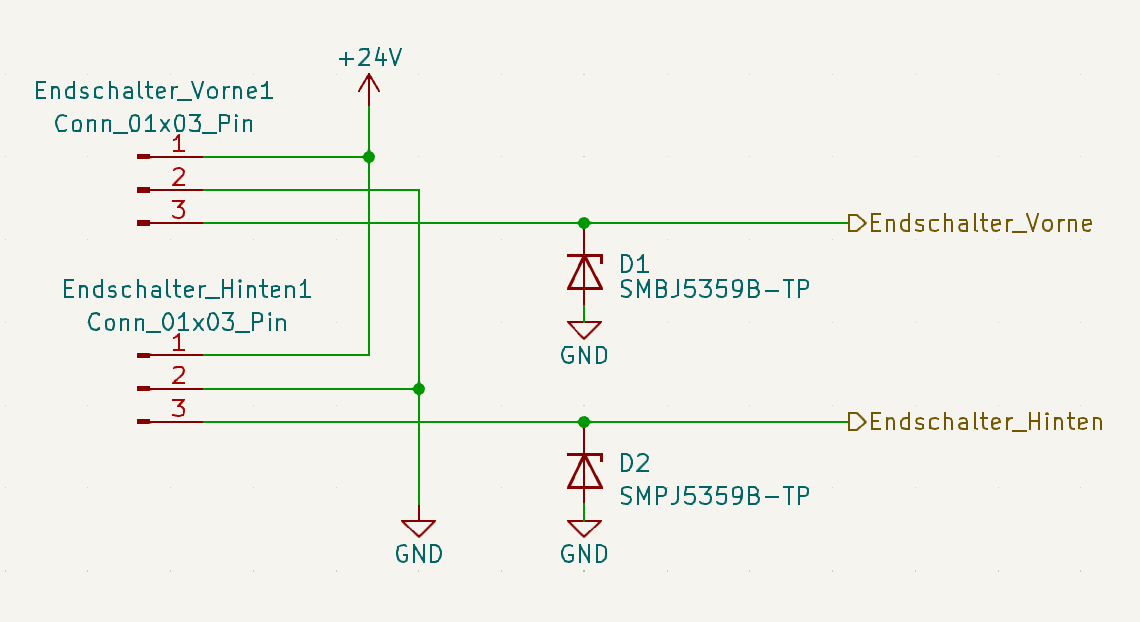
\includegraphics[width=1.0\textwidth]{images/Hardware/Endschalter_Schaltplan.PNG}
	\caption{Schaltplan der Endschalter Gruppe}
	\label{fig:EndschalterGruppe}\begin{center}
	\end{center}
\end{figure}´
\section{Bauteilliste}
\label{sec:Bauteilliste}
% Please add the following required packages to your document preamble:
% \usepackage{graphicx}
\begin{table}[H]
	\centering
	\resizebox{\textwidth}{!}{%
		\begin{tabular}{|l|l|l|}
			\hline
			\textbf{Bauteilbezeichnung} & \textbf{Bauteilart} & \textbf{Anzahl} \\ \hline
			Schurter TASTER 1104 GN & Button, Grün & 1 \\ \hline
			Schurter TASTER 1104 SW & Button, Schwarz & 2 \\ \hline
			LM3940IMP-3.3/NOPBCT-ND & Festspannungsregler & 1 \\ \hline
			FM25L16B-GTRCT-ND & F-RAM & 1 \\ \hline
			C1Q 4 & Fuse 1206, 4A & 1 \\ \hline
			3413.0223.22 & Fuse 1206, 5A & 1 \\ \hline
			RP1465 & Gehäuse & 1 \\ \hline
			R-78E5.0-0.5 & DC/DC Wandler & 1 \\ \hline
			Phoenix Contact 1984617 & Schraubterminal 2 Fach 3.5mm & 2 \\ \hline
			OSTVN02A150 & Schraubterminal 2 Fach 2.54mm & 3 \\ \hline
			OSTVN03A150 & Schraubterminal 3 Fach 2.54mm & 4 \\ \hline
			TE Connectivity 282834-7 & Schraubterminal 7 Fach  2.54mm & 1 \\ \hline
			OSTVN10A150 & Schraubterminal 10 Fach 2.54mm & 1 \\ \hline
			LM2904QS-13DICT-ND & Operationsverstärker & 1 \\ \hline
			MAX3485CSA+CT-ND & RS-485 Converter & 1 \\ \hline
			TMCS1101A3BQDRQ1CT-ND & Stromsensor & 1 \\ \hline
			LTST-C150GKT & SMD LED Grün & 3 \\ \hline
			LTST-C150KSKT & SMD LED Gelb & 3 \\ \hline
			LTST-C230KRKT & SMD LED Rot & 1 \\ \hline
			LTST-C230KFKT & SMD LED Orange & 1 \\ \hline
			LTV-817S & Optokoppler & 9 \\ \hline
			G6S-2F 24DC & Relais, 24V & 2 \\ \hline
			KDZVTR24BCT-ND & Zenerdiode, 24V & 9 \\ \hline
			Schurter FRONTSATZ & Button, Montagesatz & 3 \\ \hline
			C6000ALBB & Schalter & 1 \\ \hline
			C6000ALBB-1229W & Schalter, gekennzeichnet & 1 \\ \hline
			SL 2X10G SMD2,54 & Pin-Header, SMD & 1 \\ \hline
			SL 2X50G 2,54 & Pin-Header & 1 \\ \hline
			MEN 1216.1001 & LED-Lichtleiter & 8 \\ \hline
			KDZVTR6.8B & Zenerdiode, 6.8V & 4 \\ \hline
			IPG-2227 & Kabelverschraubung 3mm-6mm & 4 \\ \hline
			IPG-222135 & Kabelverschraubung 6mm-12mm & 4 \\ \hline
		\end{tabular}%
	}
	\caption{Bauteilliste Teil 1}
	\label{tab:Verwendeten Bauteile}
\end{table}

\begin{table}[H]
	\centering
	\begin{tabular}{|l|l|}
		\hline
		\textbf{Widerstände SMD1206} & \textbf{Anzahl} \\ \hline
		150$\Omega$ & 7 \\ \hline
		10k$\Omega$ & 5 \\ \hline
		120$\Omega$ & 4 \\ \hline
		750$\Omega$ & 2 \\ \hline
		240$\Omega$ & 1 \\ \hline
		700$\Omega$ & 6 \\ \hline
		11k$\Omega$ & 6 \\ \hline
		2,2k$\Omega$ & 3 \\ \hline
		6,8k$\Omega$ & 3 \\ \hline
		36k$\Omega$ & 3 \\ \hline
		110$\Omega$ & 1 \\ \hline
		2,3k$\Omega$ & 1 \\ \hline
		1k$\Omega$ & 1 \\ \hline
		\textbf{Kondensatoren SMD1206} &  \\ \hline
		22$\mu$F & 1 \\ \hline
		22nF & 6 \\ \hline
		220nF & 3 \\ \hline
		33$\mu$F & 1 \\ \hline
		0.47$\mu$F & 1 \\ \hline
	\end{tabular}
	\caption{Bauteilliste Teil 2}
	\label{tab:Bauteile2}
\end{table}
\newpage
\section{Valide URL und JSON Formate}
\label{sec:REST}
\subsection{GET-Anfragen}
\subsubsection{GET /data}
\begin{lstlisting}[language=XML, caption={GET-Request 1}]
{
	"error": <(int) error_code>,
	"operating_mode": <(int) 0/1 [manual/automatic]>,
	"localized": <(boolean)>,
	"sail_pos": <(int) pitch/roll [+/- 0...100 %]>,
	"wind": {
		"speed": <(int) speed[m/s]>,
		"direction": <(int) direction[degree]>
	},
	"current": <(int) current[mA]>
}
\end{lstlisting}
\subsubsection{GET /data/status}
\begin{lstlisting}[language=XML, caption={GET-Request 2}]
	{
		"error": <(int) error_code>,
		"operating_mode": <(int) 0/1 [manual/automatic]>,
		"localized": <(boolean)>,
	}
\end{lstlisting}
\subsubsection{GET /data/adjustment}
\begin{lstlisting}[language=XML, caption={GET-Request 3}]
	{
		"sail_pos": <(int) pitch/roll [+/- 0...100 %]>
	}
\end{lstlisting}
\newpage
\subsubsection{GET /data/sensors}
\begin{lstlisting}[language=XML, caption={GET-Request 4}]
	{
		"wind": {
			"speed": <(int) speed[m/s]>,
			"direction": <(int) direction[degree]>
		},
		"current": <(int) current[mA]>
	}
\end{lstlisting}
\subsubsection{GET /data/settings}
\begin{lstlisting}[language=XML, caption={GET-Request 5}]
	{
		"max_rpm": <(int) 400 - 2000>,
		"max_distance_error": <(int) 5 - 50>
	}
\end{lstlisting}

\subsection{PUT-Anfragen}
\subsubsection{PUT /data/status/error}
\begin{lstlisting}[language=XML, caption={PUT-Request 1}]
	{
		"error": <(int) error_code>,
	}
\end{lstlisting}
\newpage
\subsubsection{PUT /data/adjustment}
\begin{lstlisting}[language=XML, caption={PUT-Request 2}]
	{
		"sail_pos": <(int) pitch/roll [+/- 0...100 %]>
	}
\end{lstlisting}
\subsubsection{PUT /data/status/operating\_mode}
\begin{lstlisting}[language=XML, caption={PUT-Request 3}]
	{
		"operating_mode": <(int) 0/1 [manual/automatic]>
	}
\end{lstlisting}
\subsubsection{PUT /data/settings}
\begin{lstlisting}[language=XML, caption={PUT-Request 4}]
	{
		"max_rpm": <(int) 400 - 2000>,
		"max_distance_error": <(int) 5 - 50>
	}
\end{lstlisting}

\end{document}                                  
